\subsection{题目描述}
\noindent Write a code to numerically solve the radial Schrödinger equation for
\[
    \left[-\frac{1}{2}\nabla^2+V(\mathbf{r})\right]\psi(\mathbf{r})=E\psi(\mathbf{r}), \quad V(\mathbf{r})=V(r)
\]
\begin{enumerate}
    \item \( V(r) = \frac{1}{r} \) (hydrogen atom)
    \item Considering the following potential:
          \[
              V(r) = -\frac{Z_{\text{ion}}}{r}\text{erf}\left(\frac{r}{\sqrt{2} r_{\text{loc}}}\right)
              + \exp \left[ -\frac{1}{2} \left(\frac{r}{r_{\text{loc}}}\right)^{2}\right]
              \times \left[C_1 + C_2\left(\frac{r}{r_{\text{loc}}}\right)^2+C_3\left(\frac{r}{r_{\text{loc}}}\right)^4+C_4\left(\frac{r}{r_{\text{loc}}}\right)^6\right]
          \]
\end{enumerate}
where \(\text{erf}\) is the error function. And for Li, you could set:
\begin{itemize}
    \item \( Z_{\text{ion}}=3 \)
    \item \( r_{\text{loc}}=0.4 \)
    \item \( C_1=-14.0093922 \)
    \item \( C_2=9.5099073 \)
    \item \( C_3=-1.7532723 \)
    \item \( C_4=0.0834586 \)
\end{itemize}
\noindent Compute and plot the first three eigenstates. You could find more information about 'how to solve radial Schrödinger equation' and 'use of non-uniform grid (optional)' in the PPT.

\textbf{Special Note:} You may call any library functions for diagonalization.


\subsection{程序描述}
本程序拥有四个模块:\texttt{utils},\texttt{solver},\texttt{analysis},\texttt{visualization},分别为工具函数和配置参数模块、数值求解算法模块、结果分析和处理模块与可视化处理模块。主程序入口\texttt{main}中有主求解器类\texttt{RadialSchrodingerSolver},其计算配置与非均匀网格由\texttt{utils}中的\texttt{SolverConfig}类与\texttt{RadialGrid}类指定;势能函数调用\texttt{utils}中的\texttt{Potential}基类,其中有本题设定的氢原子库仑势与锂原子局域势,\texttt{utils}中还有一些辅助工具,在此不一一列举。主求解器的核心逻辑依赖绑定的求解器实例\texttt{ShootingSolver}或\texttt{FiniteDifferenceSolver}\footnote{Numerov实在没时间写了qwq}.主求解器还从\texttt{analysis}模块绑定了波函数处理器\texttt{WavefunctionProcessor},负责计算导数、分析波函数渐进行为、根据不同角量子数由邻域外推原点附近的波函数奇异值、归一化处理等;能量分析器\texttt{EnergyAnalyzer},负责比较能级与理论值差异;收敛性分析器\texttt{ConvergenceAnalyzer},负责分析不同网格下的收敛性。最后,来自可视化模块\texttt{visualization}中的\texttt{ResultVisualizer}负责波函数、概率密度与收敛分析结果的可视化。

采用的非均匀网格为指数网格,共$j_{\text{max}}+1$个点,参数$r_p$满足$r_{\text{max}} = r(j_{\text{max}})$,控制$j_{\text{max}} \delta =6$
\[
    r(j) =r_p (\exp(j \delta) -1)+ r_{min}, \quad j=0,1,2,\cdots, j_{\text{max}}
\]
在本题单位制$h=m=a=1$下,一维径向方程化为(注意课件上漏了个2)
\[
    u''(r) = 2(E-V_{\text{eff}}(r))u(r)
\]
此时做变换
\[
    u(j) = v(j) \exp(j \delta/2)
\]
可将方程改写为
\[
    v''(j) -\frac{\delta ^2}{4}v(j) = 2r_p^2 \delta^2 \exp(2 j \delta) (E-V_{\text{eff}}(r(j)))v(j)
\]
于是我们可以愉快地使用RK4求解了(结果示例中验证了$\mathcal{O}(h^4)$的全局误差)。一般的打靶法从原点向外积分,但此处原点附近势能奇异,故改从一个较大的$r_\text{max}$向内积分。但考虑到在$l$给定的情况下,不同能级$n$对应的演化方程相同,很可能出现求解不到指定态,或者无法收敛的情形。课件最后的参考文献\footnote{\href{https://www.iue.tuwien.ac.at/uploads/tx_sbdownloader/Bachelor-Arbeit_Marie_ERTL_09-2016.pdf}{Solving The Stationary One Dimensional Schrödinger Equation With The Shooting Method}}指出,可以对$u(r)$施加$(n - l - 1)$的节点约束,以确保求解到正确的态。但他似乎采取加一个较大的惩罚系数,如$1\mathrm{e}3*(\text{nodes}-\text{target})$,这样会使得一般的求根器容易出错,我选择改用$(\text{nodes}-\text{target})^2$,使得求解更平稳,并先在求解区间内粗扫描,再在$r_{\text{min}}$最小的值附近使用\texttt{scipy.optimize.minimize}的\texttt{l-bfgs-b}求解,在测试中发现,一些边界奇异的态需要该用\texttt{Nelder-Mead}无导数优化器,但效率与精度均下降。为了减少奇异解的发生,我还添加了波函数渐进行为约束与连续性约束,均要求在接近原点附近的几个点满足
\[
    \frac{u'(r)}{u(r)} \approx \frac{l+1}{r}
\]
不过前者是使用\([(\frac{d}{dr}\ln{u}) \cdot r -(l+1)]^2\),后者直接考虑\([u'(r)-\frac{l+1}{r}u(r)]^2\)作为权重函数,这样可以保证在原点附近的波函数行为符合物理要求。加上节点数要求与目标$u(r_\text{min})$的要求,总共四个目标函数可以加权求和作为最小化的目标,经其约束的方法大大提高了求解的稳定性与收敛性。

在有限差分法中,直接将将方程两侧除以$r_p^2 \delta^2 \exp(2 j \delta) $可以按照按照普通本征值问题求解,但实际操作发现这样的数值稳定性不太好。本程序进行两处改进,首先将$j = 0$的近核点从方程移除,其实保留也能求解,但因为该变换限制了第一个点与第二个点较近,且离心势能的$\frac{1}{r^2}$奇异会带来一些麻烦,如图\ref{fig:ill}所示
\begin{figure}
    \centering
    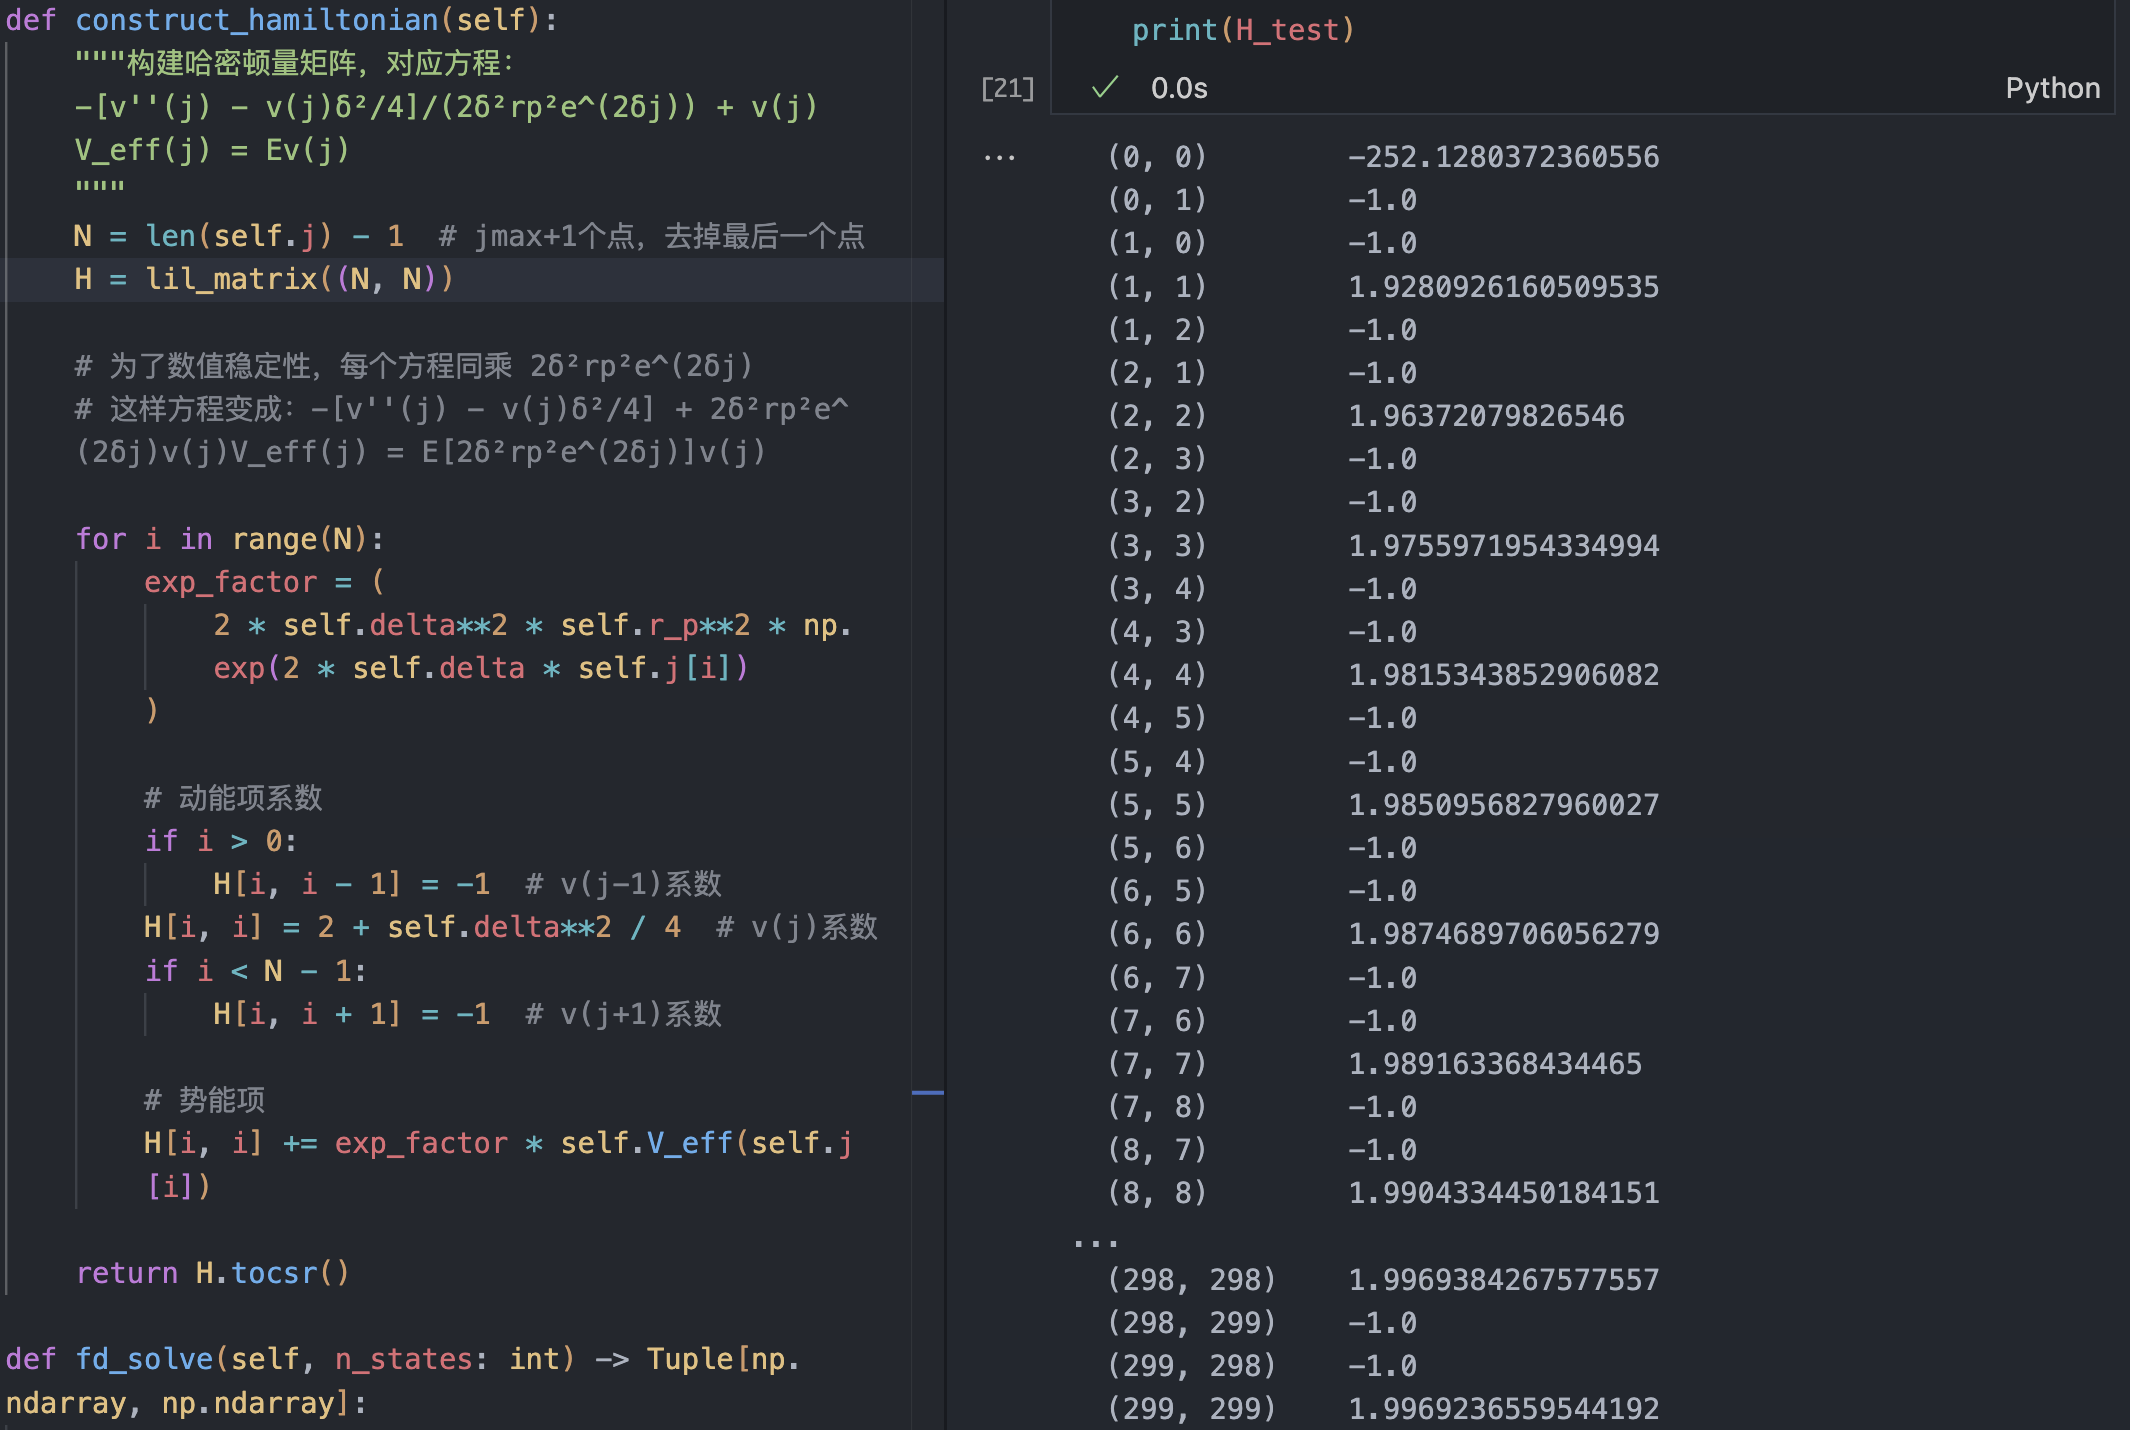
\includegraphics[width=0.8\textwidth]{Problem_2/figs/ill_h_test.png}
    \caption{去掉第一个点前的病态矩阵}
    \label{fig:ill}
\end{figure}
而我们求解的$u$总是在第一个点趋于0的,所以去掉可以提高数值稳定性。其次,我们原先的方程也是可以直接求解的,属于广义本征值问题$\mathbf{A} \mathbf{u} = \lambda \mathbf{B} \mathbf{u}$,而\texttt{scipy}内置的库对其迭代有优化,可加快收敛,只不过要构造两个系数矩阵。借助本题氢原子与类氢原子的能级$E_n \approx \frac{1}{n^2}$趋势,我还使用了shift-invert模式,即在基态的$\frac{1}{n^2}$附近找寻激发态\footnote{令人匪夷所思的是,早期版本中$j_{\text{max}}<1000$的网格基本都能收敛求解,但不知改动了哪里,现在在一些稍小网格数测试中也经常不收敛。},提高了求解速度,但在已知的3p态测试中,经常导致漏掉该态直接找寻4p态。

可在\texttt{Problem\_2/src/radial\_schrodinger}目录下运行\ccmd{pip install -e .}临时安装本包,然后导入或直接运行\ccmd{python main.py},如果不安装,也可以在\texttt{Problem\_2/src}目录下运行\ccmd{python radial\_schrodinger.py},均支持命令行参数,请加上\ccmd{-h}查看帮助信息。助教老师还可以借助\texttt{\href{https://bud-primordium.github.io/Computational-Physics-Fall-2024/Assignment_7/Problem_2/Sphinx.html}{Sphinx.html}}\footnote{Github Pages上的静态版本控制格式有些问题,本地文档可正常使用}查看本包的文档。
\subsection{伪代码}
Powered by \href{https://chatgpt.com/g/g-xJJAA2awf-latex-pseudocode-generator}{\LaTeX \ pseudocode generator}
\subsubsection{打靶法}
\begin{algorithm}[H]
    \SetAlgoLined
    \SetKwFunction{Derivative}{Derivative}
    \KwIn{$E$: Energy (float)}
    \KwOut{$u$: Normalized wavefunction array (radial grid)}
    
    Initialize $v[j_{\text{max}}] \gets 0$, $v'[j_{\text{max}}] \gets -1$ \tcp*[r]{Boundary conditions}
    Set step size $h \gets -1$ \tcp*[r]{Negative for inward integration}
    
    \For{$j \gets j_{\text{max}}-1$ \KwTo $0$}{
    Compute $(k_1^v, k_1^{v'}) \gets$ \Derivative{$j+1, v[j+1], v'[j+1]$}\;
    Compute $(k_2^v, k_2^{v'}) \gets$ \Derivative{$j+0.5, v[j+1]+0.5 \cdot h \cdot k_1^v, v'[j+1]+0.5 \cdot h \cdot k_1^{v'}$}\;
    Compute $(k_3^v, k_3^{v'}) \gets$ \Derivative{$j+0.5, v[j+1]+0.5 \cdot h \cdot k_2^v, v'[j+1]+0.5 \cdot h \cdot k_2^{v'}$}\;
    Compute $(k_4^v, k_4^{v'}) \gets$ \Derivative{$j, v[j+1]+h \cdot k_3^v, v'[j+1]+h \cdot k_3^{v'}$}\;
    
    Update $v[j] \gets v[j+1] + \frac{h}{6} \cdot (k_1^v + 2 \cdot k_2^v + 2 \cdot k_3^v + k_4^v)$\;
    Update $v'[j] \gets v'[j+1] + \frac{h}{6} \cdot (k_1^{v'} + 2 \cdot k_2^{v'} + 2 \cdot k_3^{v'} + k_4^{v'})$\;
    }
    
    Transform $u \gets v \cdot \exp(\delta \cdot j / 2)$ \tcp*[r]{Transform to radial wavefunction}
    Normalize $u$ if $\|u\| > 0$ \tcp*[r]{Ensure normalization}
    \KwRet{$u$}
    \caption{Inward Integration with RK4}
\end{algorithm}

\begin{algorithm}[H]
    \SetAlgoLined
    \SetKwFunction{Integrate}{IntegrateInward}
    \KwIn{$E$: Energy (float)}
    \KwOut{$\text{Error}$: Objective function value}
    
    Compute $u \gets$ \Integrate{$E$} \tcp*[r]{Solve radial Schrödinger equation}
    Compute $r$, $u'$ \tcp*[r]{Radial positions and derivatives}
    
    \BlankLine
    \textbf{Step 1: Logarithmic Derivative Error} \tcp*[r]{Near $r_{\min}$}
    Compute $\text{LogDerError}$ based on $u$ and $u'$ \tcp*[r]{Match theoretical values}
    
    \BlankLine
    \textbf{Step 2: Node Count Error} \tcp*[r]{Compare nodes with target}
    Compute $\text{NodesError}$ based on node difference\;
    
    \BlankLine
    \textbf{Step 3: Amplitude Error at $r_{\min}$}\;
    Compute $\text{AmpError} \gets u[0]^2$\;
    
    \BlankLine
    \textbf{Step 4: Continuity Error}\;
    Compute $\text{ContError} \gets (u'[0] - \text{TheoreticalDerivative})^2$\;
    
    Compute $\text{TotalError} \gets w_1 \cdot \text{LogDerError} + w_2 \cdot \text{NodesError} + w_3 \cdot \text{AmpError} + w_4 \cdot \text{ContError}$\;
    
    \KwRet{$\text{TotalError}$}
    \caption{Objective Function for Energy Optimization}
\end{algorithm}
\begin{algorithm}[H]
    \SetAlgoLined
    \SetKwFunction{Objective}{Objective}
    \SetKwFunction{Integrate}{IntegrateInward}
    \SetKwFunction{Optimize}{Minimize}
    \SetKwFunction{Raise}{Raise}
    \KwIn{$E_{\min}$, $E_{\max}$: Energy bounds, $N_{\text{target}}$: Target node count}
    \KwOut{$E_{\text{optimal}}$: Optimal energy, $u$: Normalized wavefunction}
    
    Set $N_{\text{target}} \gets n - l - 1$ if not specified\;
    Define weights $w_1, w_2, w_3, w_4$ for multi-objective terms\;
    
    \BlankLine
    \textbf{Step 1: Coarse Grid Search}\;
    Generate energy grid $E_{\text{grid}} \in [E_{\min}, E_{\max}]$\;
    Compute errors $\text{Errors}[i] \gets$ \Objective{$E_{\text{grid}}[i]$}\;
    Set $E_{\text{coarse}} \gets \arg\min(\text{Errors})$\;
    
    \BlankLine
    \textbf{Step 2: Fine Optimization}\;
    Perform optimization $\text{Result} \gets$ \Optimize{$\text{Objective}$, initial guess $E_{\text{coarse}}$}\;
    
    \If{$\text{Result.success}$}{
        Compute $u_{\text{optimal}} \gets$ \Integrate{$E_{\text{optimal}}$}\;
        \KwRet{$E_{\text{optimal}}, u_{\text{optimal}}$}\;
    }
    \Else{
        \Raise{RuntimeError: Optimization did not converge}
    }
    
    \caption{Shooting Method for Energy Eigenvalue and Wavefunction}
\end{algorithm}
\subsubsection{有限差分法}
\begin{algorithm}[H]
    \SetAlgoLined
    \SetKwFunction{Veff}{V\_eff}
    \KwOut{$H$: Sparse Hamiltonian matrix}
    
    Initialize $H$ as a sparse matrix with size $(N_{\text{reduced}}, N_{\text{reduced}})$ \tcp*[r]{Reduced grid size}
    \For{$i \gets 0$ \KwTo $N_{\text{reduced}} - 1$}{
        Compute $j_{\text{actual}} \gets i + 1$ \tcp*[r]{Actual grid index}
        Compute $\text{exp\_factor} \gets 2 \cdot \delta^2 \cdot r_p^2 \cdot \exp(2 \cdot \delta \cdot j_{\text{actual}})$\;
        
        \If{$i > 0$}{Set $H[i, i-1] \gets -1$ \tcp*[r]{Kinetic term for $j-1$}}
        Set $H[i, i] \gets 2 + \frac{\delta^2}{4} + \text{exp\_factor} \cdot$ \Veff{$j_{\text{actual}}$}\;
        \If{$i < N_{\text{reduced}} - 1$}{Set $H[i, i+1] \gets -1$ \tcp*[r]{Kinetic term for $j+1$}}
    }
    \KwRet{$H$}
    \caption{Construct Hamiltonian Matrix}
\end{algorithm}
\begin{algorithm}[H]
    \SetAlgoLined
    \KwOut{$B$: Sparse matrix for scaling factors}
    
    Initialize $B$ as a sparse matrix with size $(N_{\text{reduced}}, N_{\text{reduced}})$\;
    \For{$i \gets 0$ \KwTo $N_{\text{reduced}} - 1$}{
        Compute $j_{\text{actual}} \gets i + 1$\;
        Set $B[i, i] \gets 2 \cdot \delta^2 \cdot r_p^2 \cdot \exp(2 \cdot \delta \cdot j_{\text{actual}})$\;
    }
    \KwRet{$B$}
    \caption{Construct B Matrix}
\end{algorithm}
\begin{algorithm}[H]
    \SetAlgoLined
    \SetKwFunction{ConstructHamiltonian}{ConstructHamiltonian}
    \SetKwFunction{ConstructB}{ConstructB}
    \SetKwFunction{EigSolve}{linalg.eigsh}
    \SetKwFunction{Raise}{Raise}
    \SetKwFunction{Break}{Break}
    \SetKwBlock{Try}{Try}{EndTry}
    \SetKwBlock{Catch}{Catch}{EndCatch}
    
    \KwIn{$n_{\text{states}}$: Number of eigenstates to compute}
    \KwOut{$(\text{energies}, \text{u\_states})$: Eigenvalues and normalized wavefunctions}
    
    Set $H \gets$ \ConstructHamiltonian{}\;
    Set $B \gets$ \ConstructB{$H.\text{shape}[0]$}\;
    
    \BlankLine
    \textbf{Step 1: Compute Ground State}\;
    \Try{
        Compute $(e_{\text{ground}}, v_{\text{ground}}) \gets$ \EigSolve{$H$, $k=1$, $M=B$, $which="SA"$}\;
    }
    \Catch{Exception $e$}{
        \Raise{RuntimeError: Ground state computation failed}\;
    }
    Set $\text{energies} \gets [e_{\text{ground}}]$, $\text{states} \gets [v_{\text{ground}}]$\;
    
    \BlankLine
    \textbf{Step 2: Compute Excited States (if $n_{\text{states}} > 1$)}\;
    \For{$n \gets 2$ \KwTo $n_{\text{states}}$}{
    Compute $\text{estimated\_e} \gets e_{\text{ground}} / n^2$ \tcp*[r]{Estimate using $1/n^2$ scaling}
    Set $\text{window} \gets |e_{\text{ground}}| \cdot 0.1$\;
    \ForEach{$\text{shift} \in \{\text{estimated\_e}, \text{estimated\_e} \pm \text{window}\}$}{
        \Try{
            Compute $(e, v) \gets$ \EigSolve{$H$, $k=1$, $M=B$, $\sigma=\text{shift}$, $which="LM"$}\;
            \If{$|e - e_{\text{prev}}| > 1e^{-6}$ for all $e_{\text{prev}} \in \text{energies}$}{
                Append $e$ to $\text{energies}$, $v$ to $\text{states}$\;
                \Break\; % Exit the inner loop if successful
            }
        }
        \Catch{Exception $e$}{
            Continue to the next $\text{shift}$ \tcp*[r]{Skip this shift on failure}
        }
    }
    }
    
    \BlankLine
    \textbf{Step 3: Normalize Wavefunctions and Transform to $u(r)$}\;
    Set $\text{u\_states} \gets \text{Transform and normalize states}$\;
    
    \KwRet{$(\text{energies}, \text{u\_states})$}
    \caption{Finite Difference Solver for Eigenvalues and Eigenstates}
\end{algorithm}
\subsection{结果示例}
\subsubsection{打靶法计算结果}
\begin{threeparttable}
    \begin{tabular}{|c|c|c|c|c|c|}
        \hline
        原子                   & 量子数 \(n, l\)     & 能级 (单位: hartree)   & 原子                   & 量子数 \(n, l\)     & 能级 (单位: hartree)   \\ \hline
        \multirow{6}{*}{氢原子} & \(n=1, l=0, 1s\) & -0.500000          & \multirow{6}{*}{锂原子} & \(n=1, l=0, 1s\) & -4.458247          \\ \cline{2-3} \cline{5-6}
                             & \(n=2, l=0, 2s\) & -0.125000          &                      & \(n=2, l=0, 2s\) & -1.115432          \\ \cline{2-3} \cline{5-6}
                             & \(n=2, l=1, 2p\) & -0.125000          &                      & \(n=2, l=1, 2p\) & -1.122278          \\ \cline{2-3} \cline{5-6}
                             & \(n=3, l=0, 3s\) & -0.055556          &                      & \(n=3, l=0, 3s\) & -0.496256\tnote{b} \\ \cline{2-3} \cline{5-6}
                             & \(n=3, l=1, 3p\) & -0.055556\tnote{a} &                      & \(n=3, l=1, 3p\) & -0.498679          \\ \cline{2-3} \cline{5-6}
                             & \(n=3, l=2, 3d\) & -0.055556          &                      & \(n=3, l=2, 3d\) & -0.500262          \\ \hline
    \end{tabular}
    \begin{tablenotes}
        \item[a] 对于 \(n=3\) 的三个态,指定了 \texttt{r\_Max=60},精度大幅提高,但下面图片为展现边界效应未替换
        
        \item[b] 对于 \(n=3\) 的三个态,指定了 \texttt{r\_Max=60},否则无法收敛,甚至边界发散
    \end{tablenotes}
\end{threeparttable}
\subsubsection{有限差分法计算结果}
\begin{threeparttable}
    \begin{tabular}{|c|c|c|c|c|c|}
        \hline
        原子                   & 量子数 \(n, l\)     & 能级 (单位: hartree)   & 原子                   & 量子数 \(n, l\)     & 能级 (单位: hartree)   \\ \hline
        \multirow{6}{*}{氢原子} & \(n=1, l=0, 1s\) & -0.499993          & \multirow{6}{*}{锂原子} & \(n=1, l=0, 1s\) & -4.458266\tnote{d} \\ \cline{2-3} \cline{5-6}
                             & \(n=2, l=0, 2s\) & -0.125007          &                      & \(n=2, l=0, 2s\) & -1.115469          \\ \cline{2-3} \cline{5-6}
                             & \(n=2, l=1, 2p\) & -0.125003          &                      & \(n=2, l=1, 2p\) & -1.122296          \\ \cline{2-3} \cline{5-6}
                             & \(n=3, l=0, 3s\) & -0.055556\tnote{a} &                      & \(n=3, l=0, 3s\) & -0.496337          \\ \cline{2-3} \cline{5-6}
                             & \(n=3, l=1, 3p\) & -0.031255\tnote{b} &                      & \(n=3, l=1, 3p\) & -0.280662\tnote{e} \\ \cline{2-3} \cline{5-6}
                             & \(n=3, l=2, 3d\) & -0.055529\tnote{c} &                      & \(n=3, l=2, 3d\) & -0.500269\tnote{f} \\ \hline
    \end{tabular}
    \begin{tablenotes}
        \item[a] 在\texttt{r\_Max=30}偏差过大,提升至60
        \item[b] 实际上是4p态,但始终找不到正确的3p,可能是窗口设置太小
        \item[c] 3d态在\texttt{r\_Max=30}表现尚好,因其极大值离核,边界效应不显著
        \item[d] 使用\texttt{r\_Max=30},\texttt{j\_Max=300},表现良好 
        \item[e] 实际上应该是4p态,但也始终找不到正确的3p
        \item[f] 提升至\texttt{j\_Max=400}后与打靶法结果差距更小
    \end{tablenotes}
\end{threeparttable}

\subsubsection{输入与异常处理}
\begin{figure}[H]
    \centering
    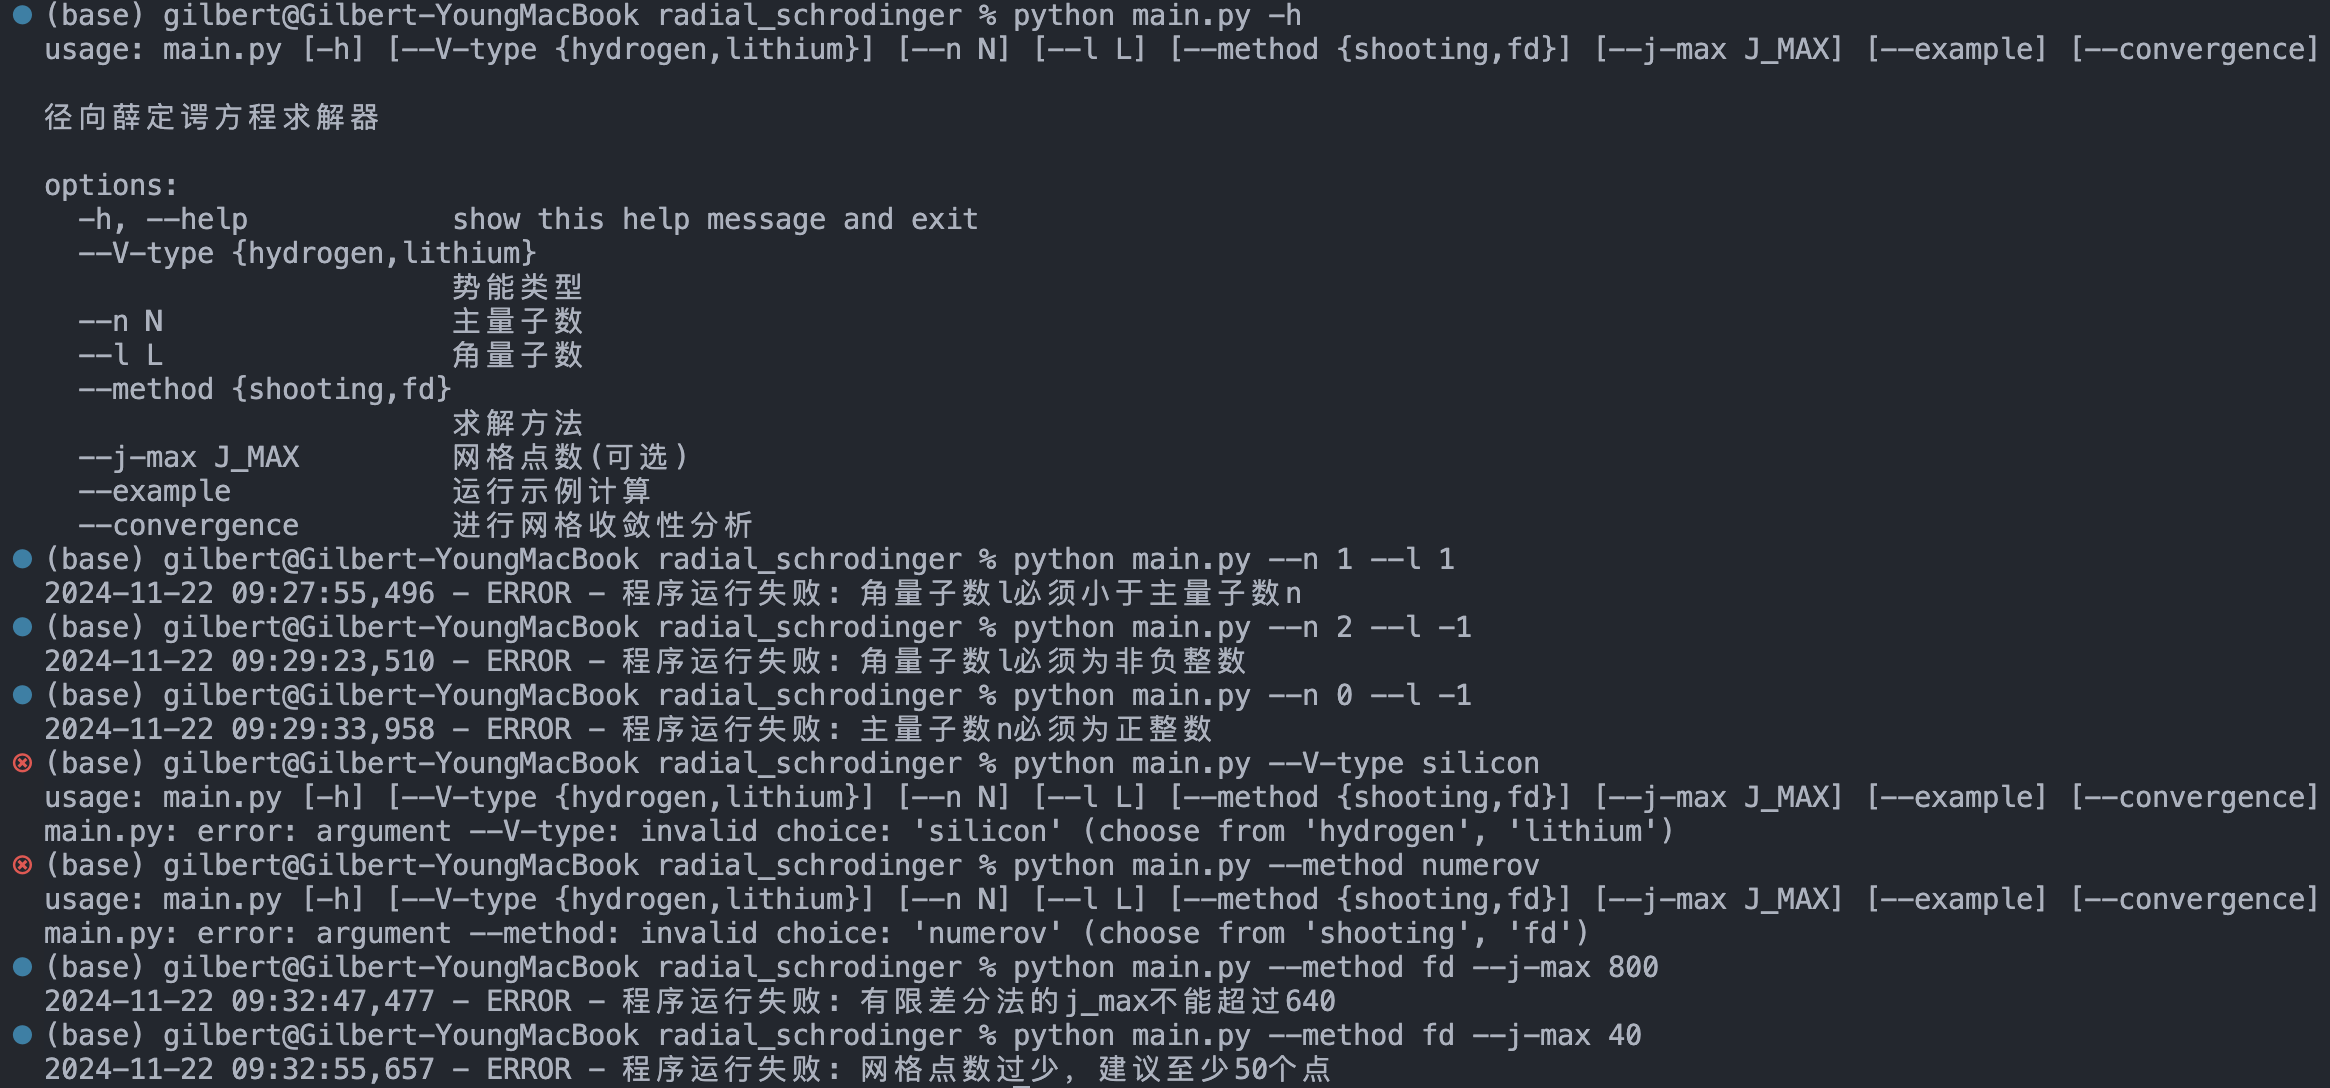
\includegraphics[width=1.0\textwidth]{Problem_2/figs/error-terminal.png}
    \caption{自定义参数输入与异常处理,新版本支持网格起止点\texttt{r\_min}与\texttt{r\_Max}的指定}
\end{figure}

\subsubsection{使用example选项运行的示例}
\begin{figure}[H]
    \centering
    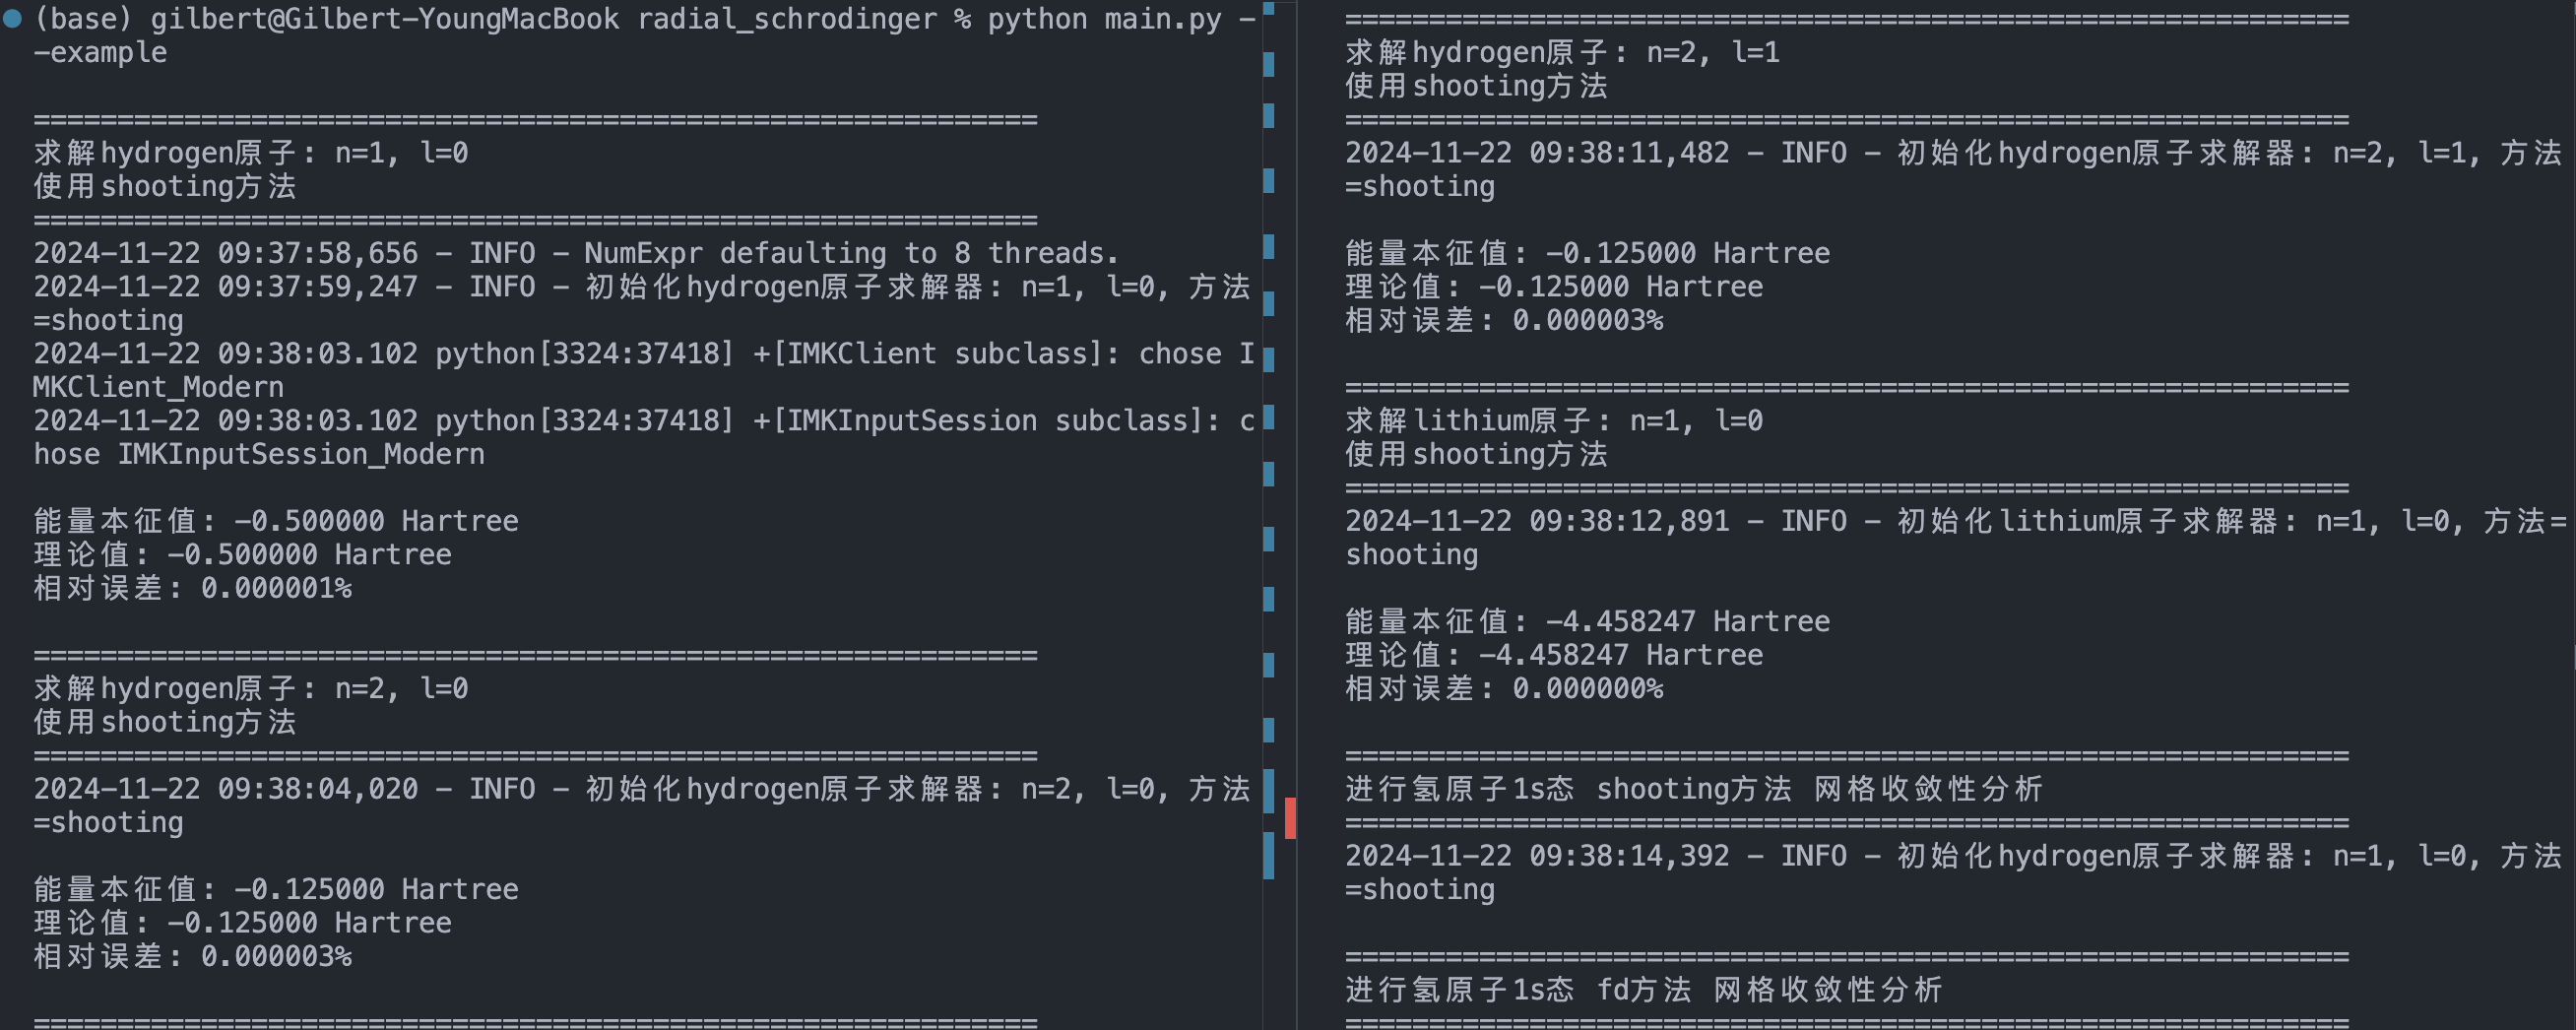
\includegraphics[width=1.0\textwidth]{Problem_2/figs/example-terminal.png}
    \caption{运行示例的终端输出}
\end{figure}

\begin{figure}[H]
    \centering
    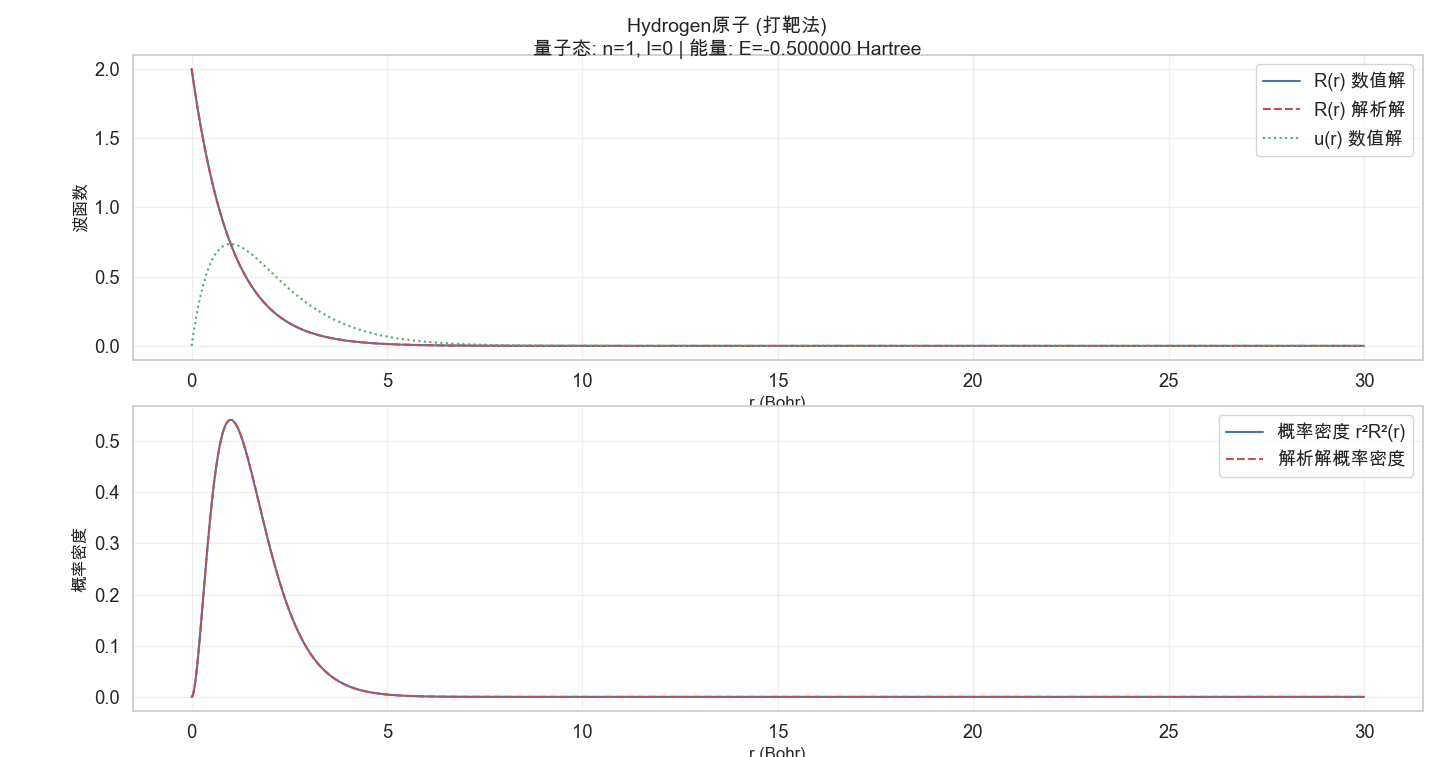
\includegraphics[width=1.0\textwidth]{Problem_2/figs/example_h_shooting_1s.png}
    \caption{使用打靶法求解氢原子库仑势的1s态}
\end{figure}

\begin{figure}[H]
    \centering
    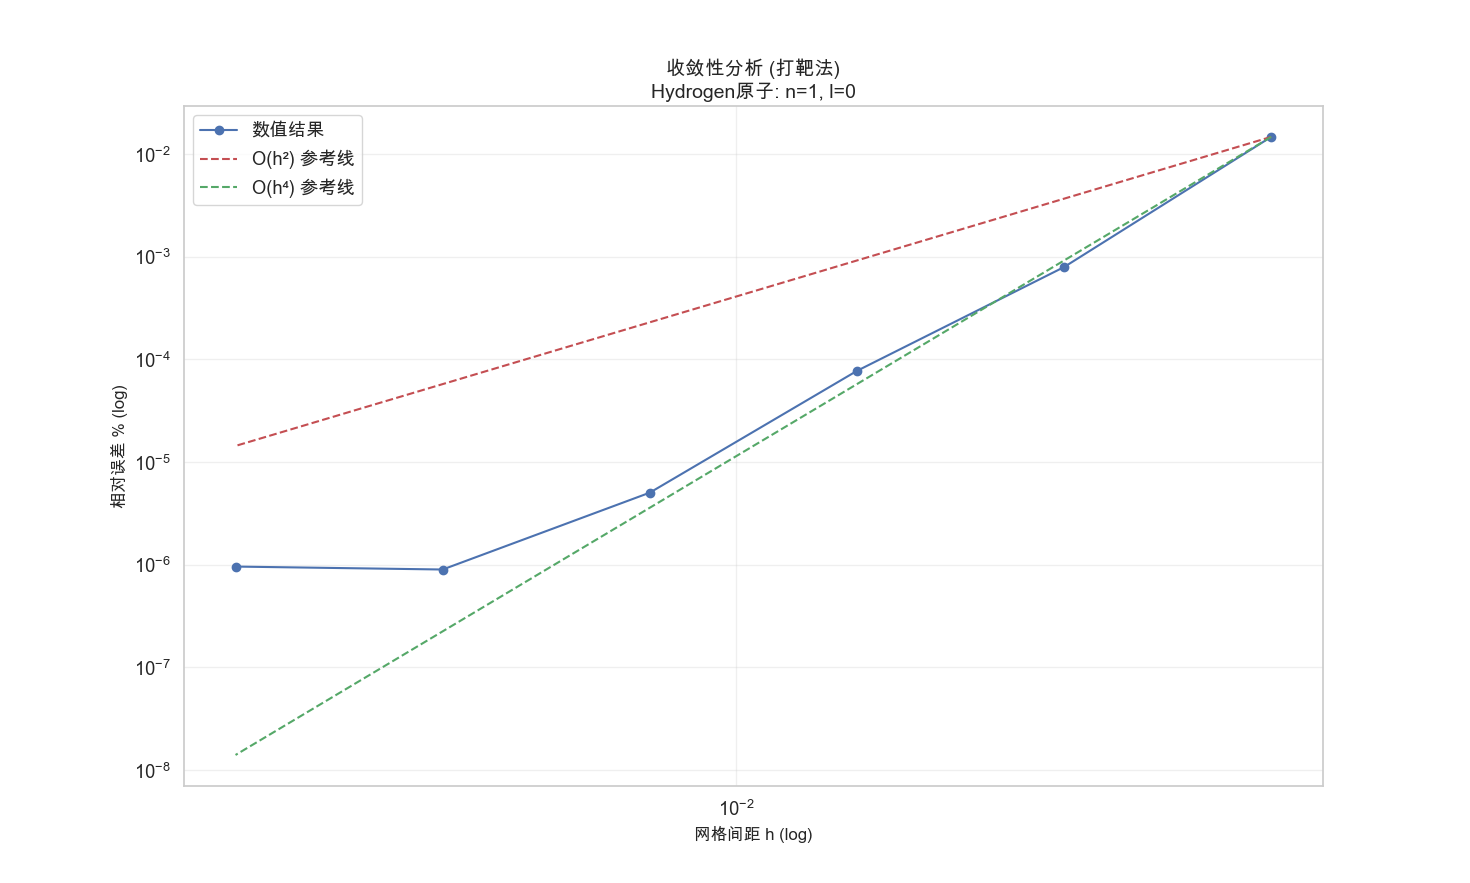
\includegraphics[width=1.0\textwidth]{Problem_2/figs/example_h_shooting_1s_con.png}
    \caption{使用打靶法求解氢原子库仑势的1s态的收敛性分析,验证了RK4全局误差是四阶精度的}
\end{figure}

\begin{figure}[H]
    \centering
    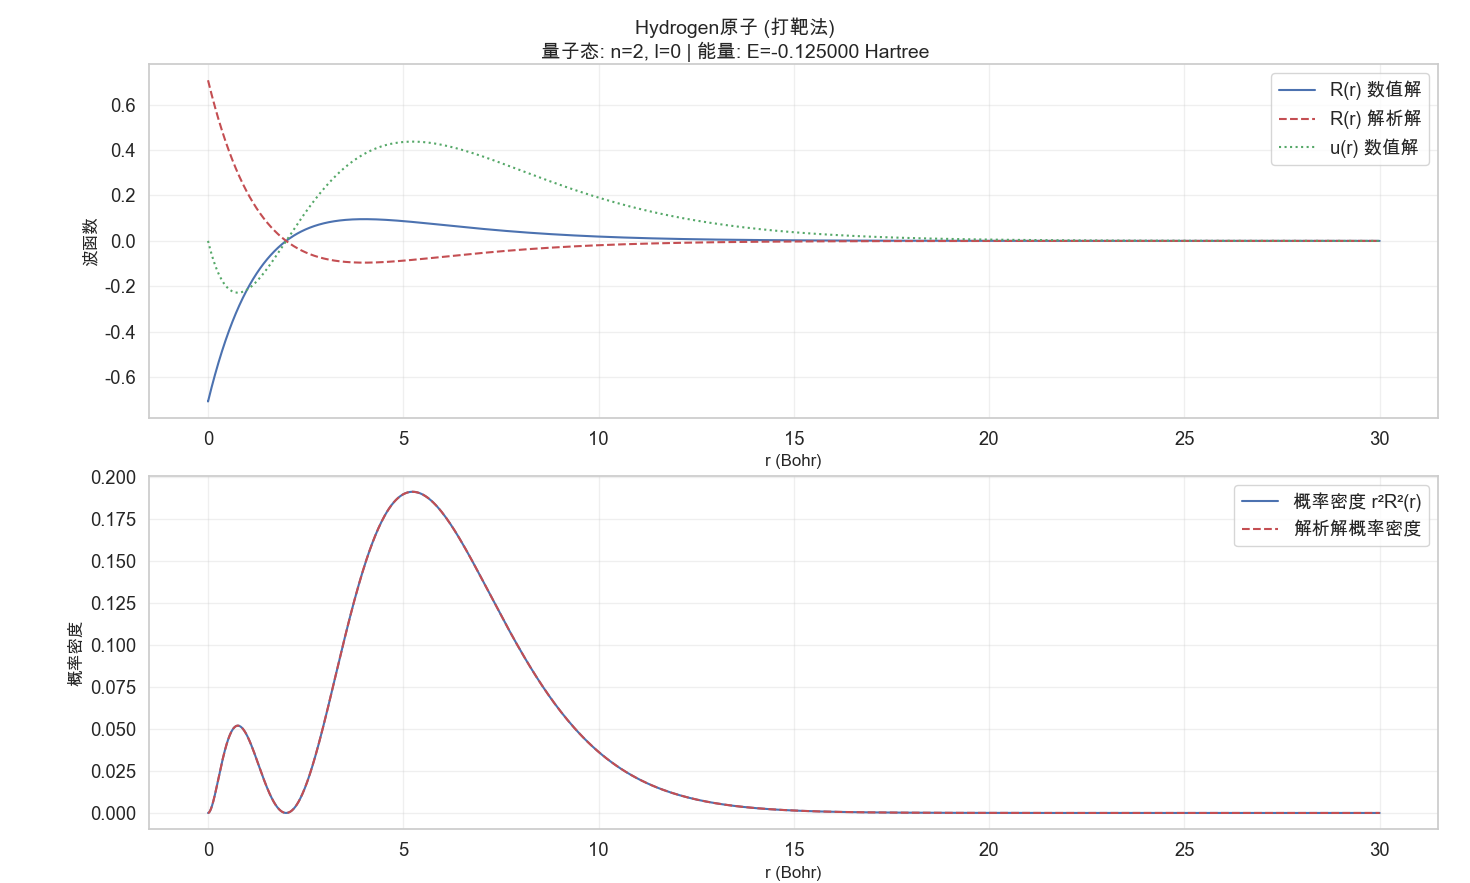
\includegraphics[width=1.0\textwidth]{Problem_2/figs/example_h_shooting_2s.png}
    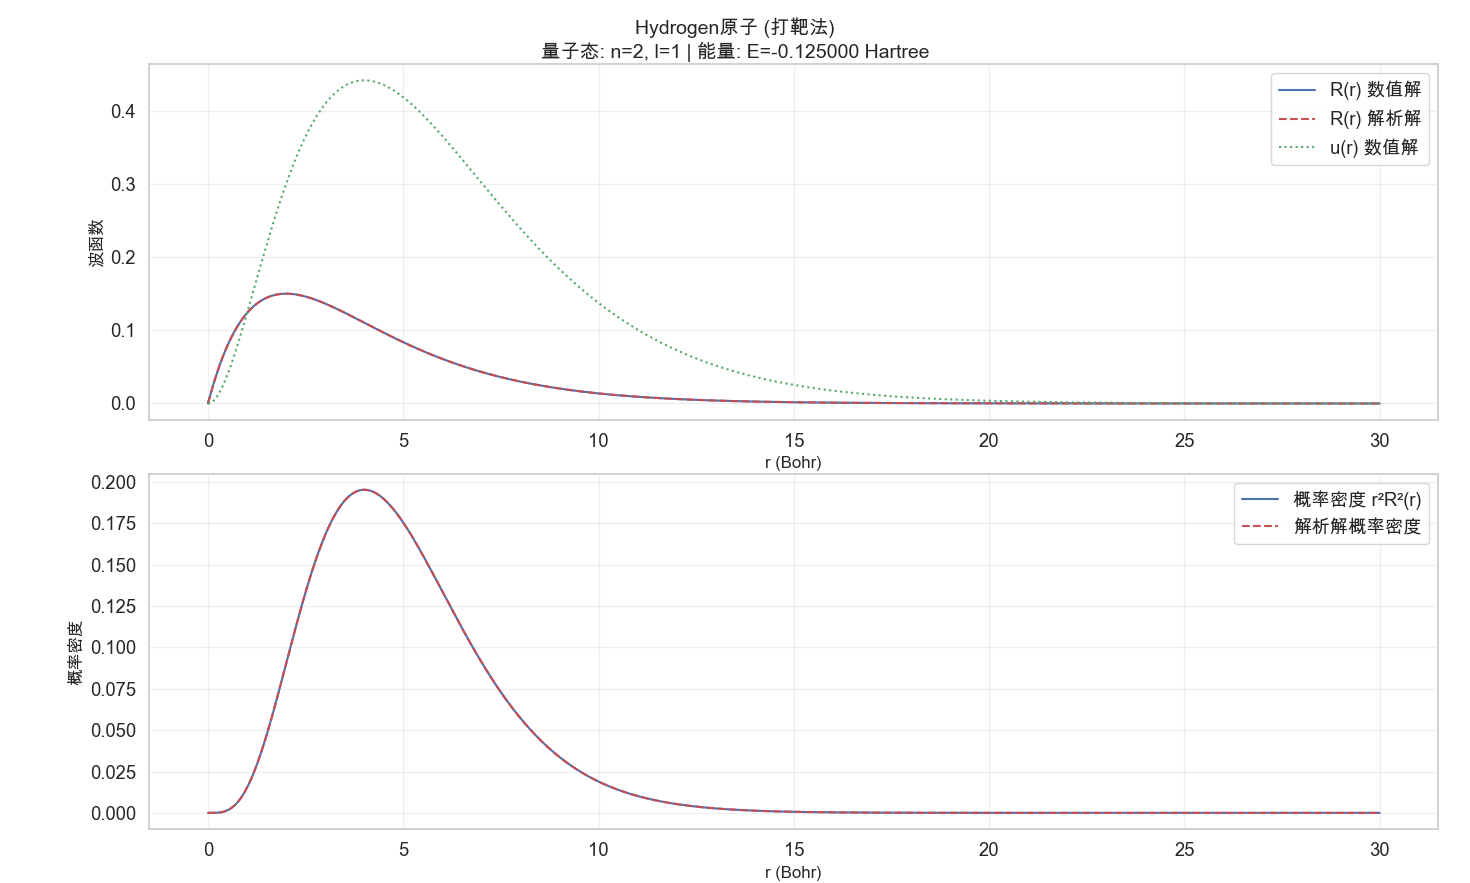
\includegraphics[width=1.0\textwidth]{Problem_2/figs/example_h_shooting_2p.png}
    \caption{使用打靶法求解氢原子库仑势的2s,2p态}
\end{figure}

\begin{figure}[H]
    \centering
    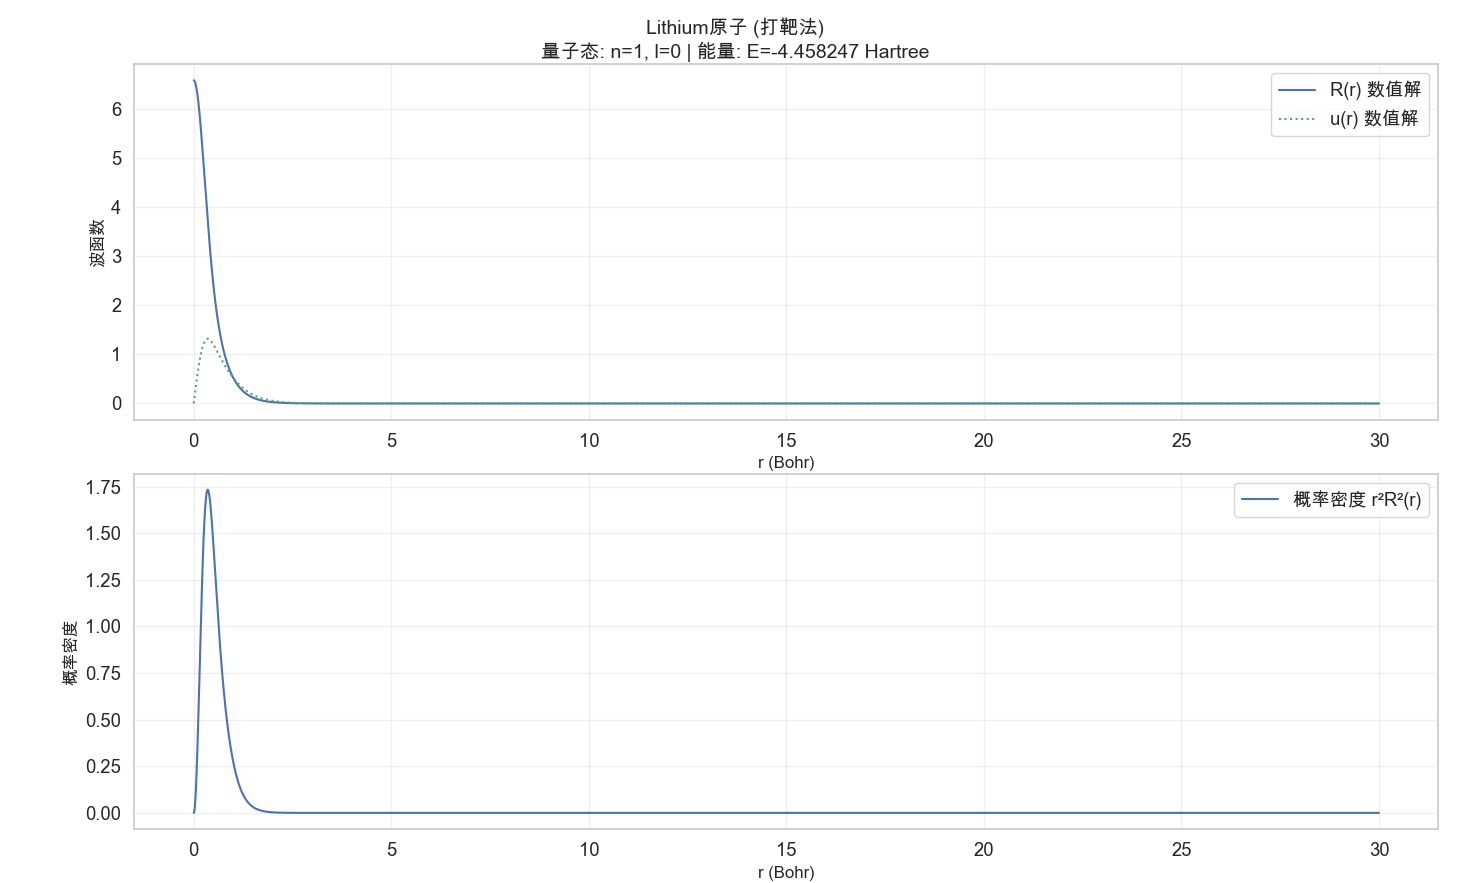
\includegraphics[width=1.0\textwidth]{Problem_2/figs/example_li_shooting_1s.png}
    \caption{使用打靶法求解锂原子局域势的1s态}
\end{figure}

\begin{figure}[H]
    \centering
    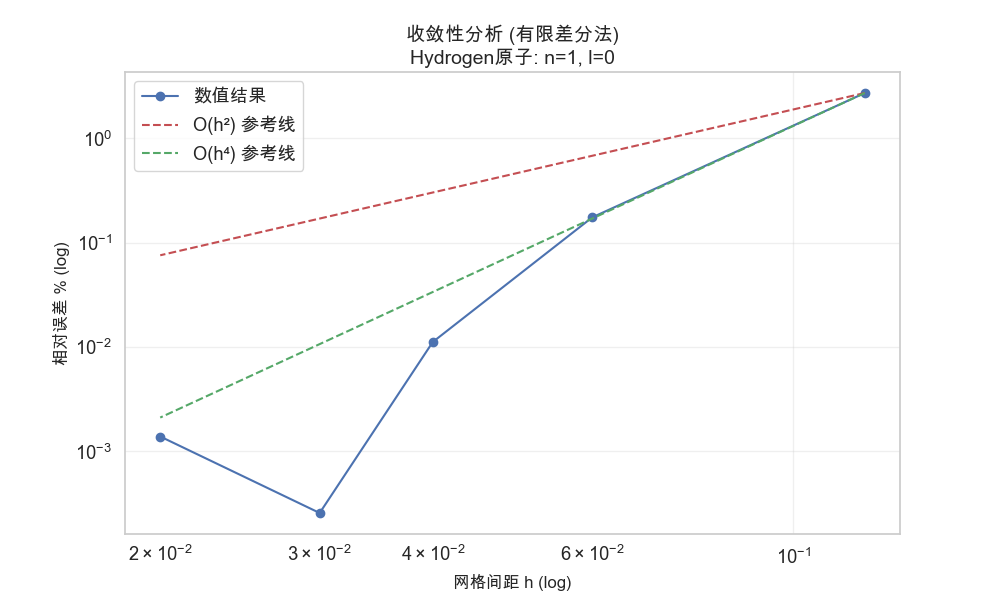
\includegraphics[width=0.8\textwidth]{Problem_2/figs/example_h_fd_1s_con.png}
    \caption{使用有限差分法求解氢原子库仑势的1s态的收敛性分析,新版本非均匀细网格的数值稳定性有所下降}
\end{figure}

\subsubsection{氢原子其它示例}
\begin{figure}[H]
    \centering
    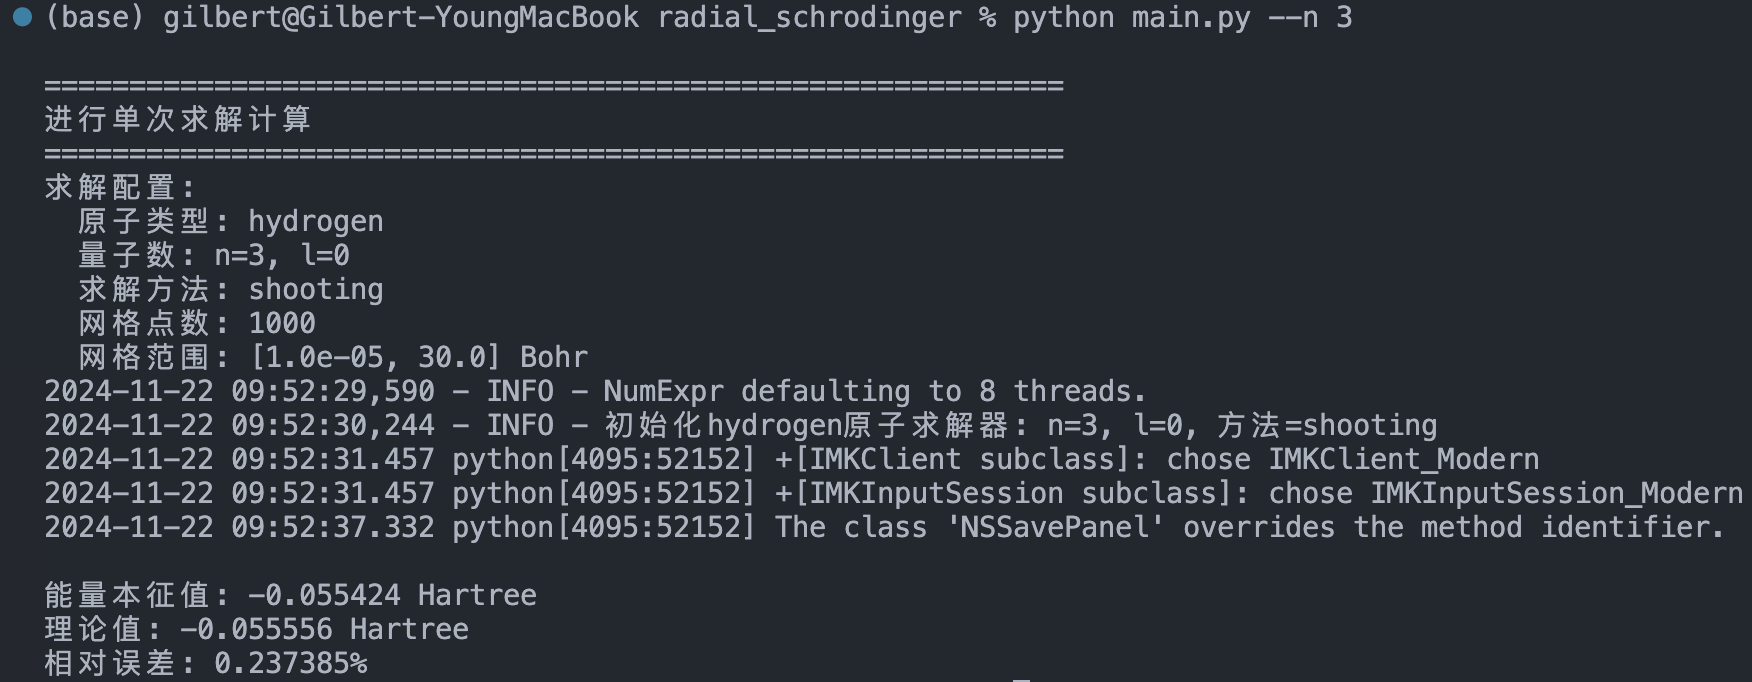
\includegraphics[width=1.0\textwidth]{Problem_2/figs/h_shooting_3s_terminal.png}
    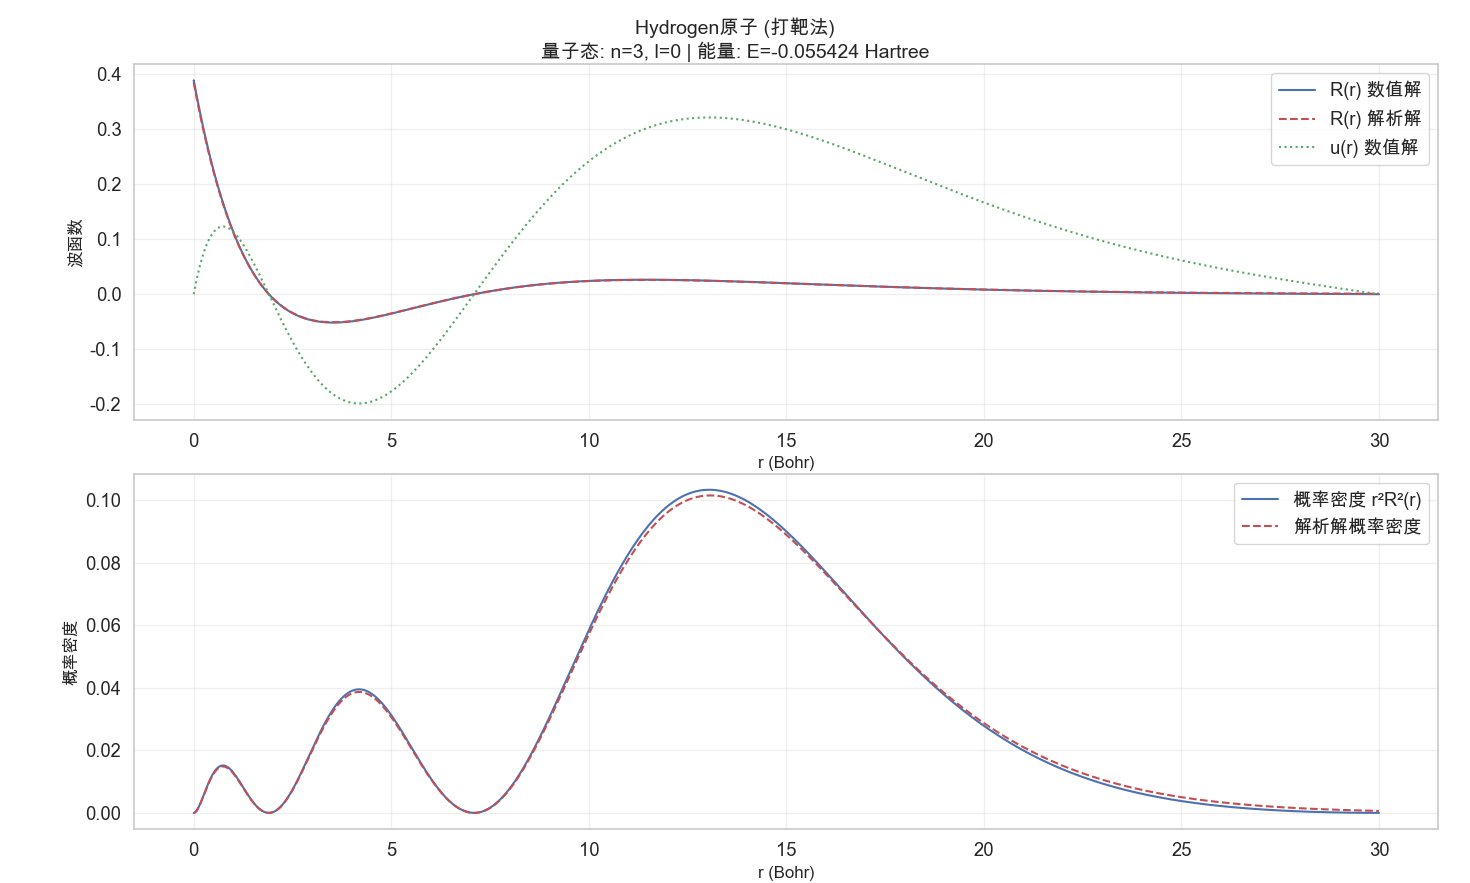
\includegraphics[width=1.0\textwidth]{Problem_2/figs/h_shooting_3s.png}
    \caption{使用打靶法求解氢原子库仑势的3s态,\texttt{r\_Max=30}的选项已经有些捉襟见肘}
\end{figure}

\begin{figure}[H]
    \centering
    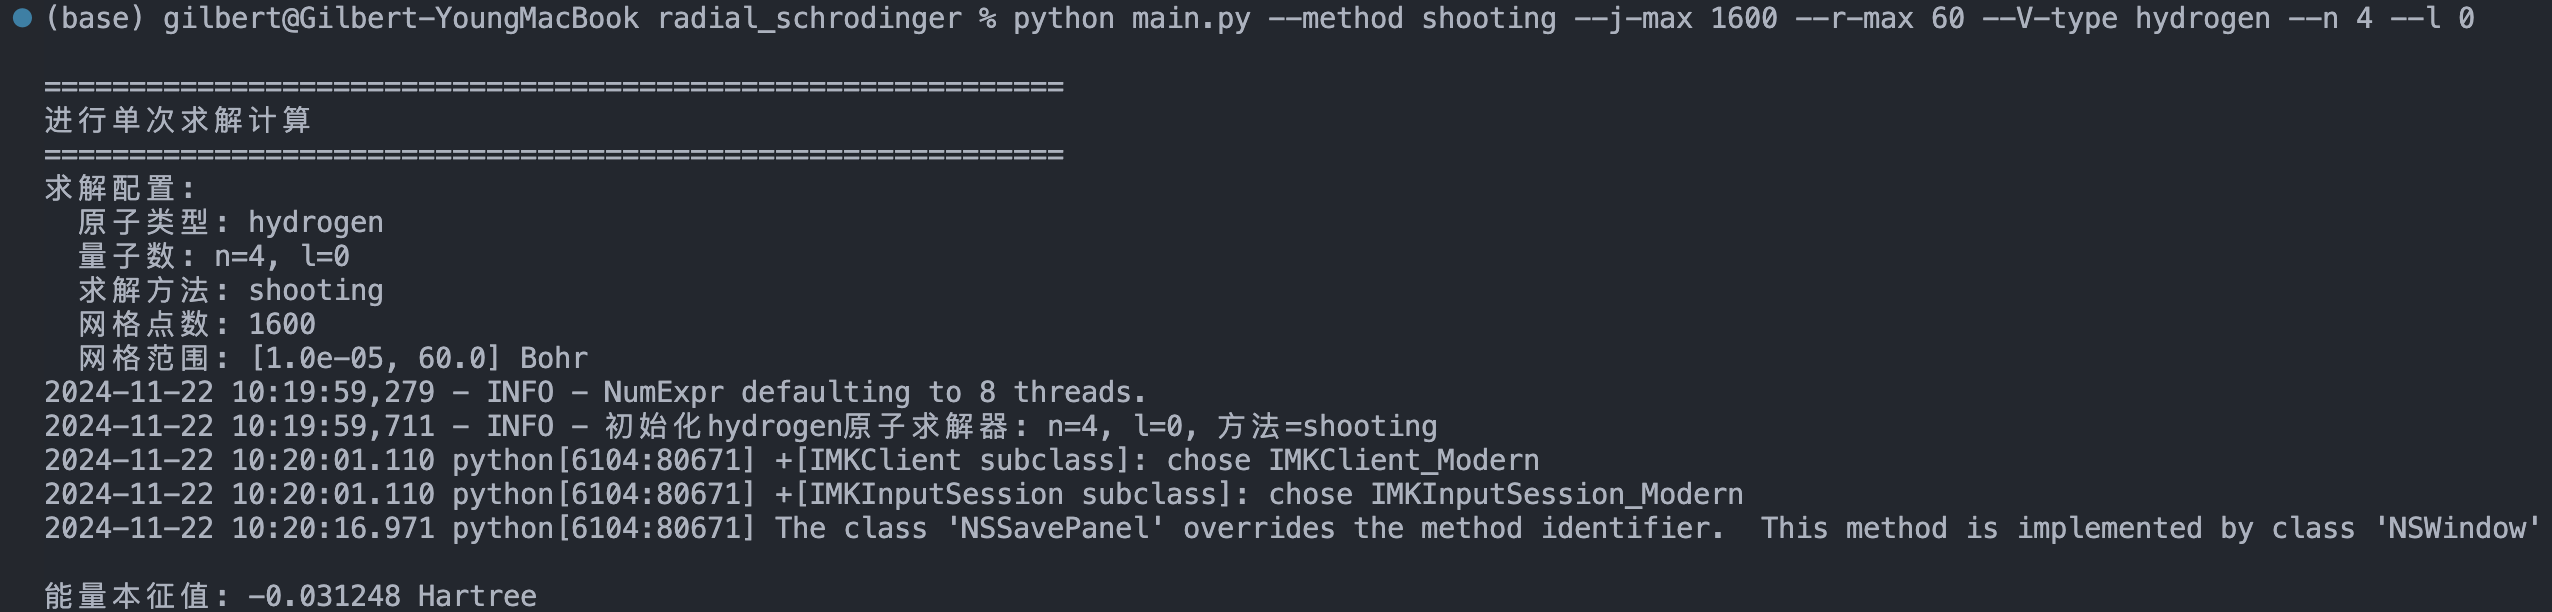
\includegraphics[width=0.6\textwidth]{Problem_2/figs/h_shooting_4s_terminal.png}
    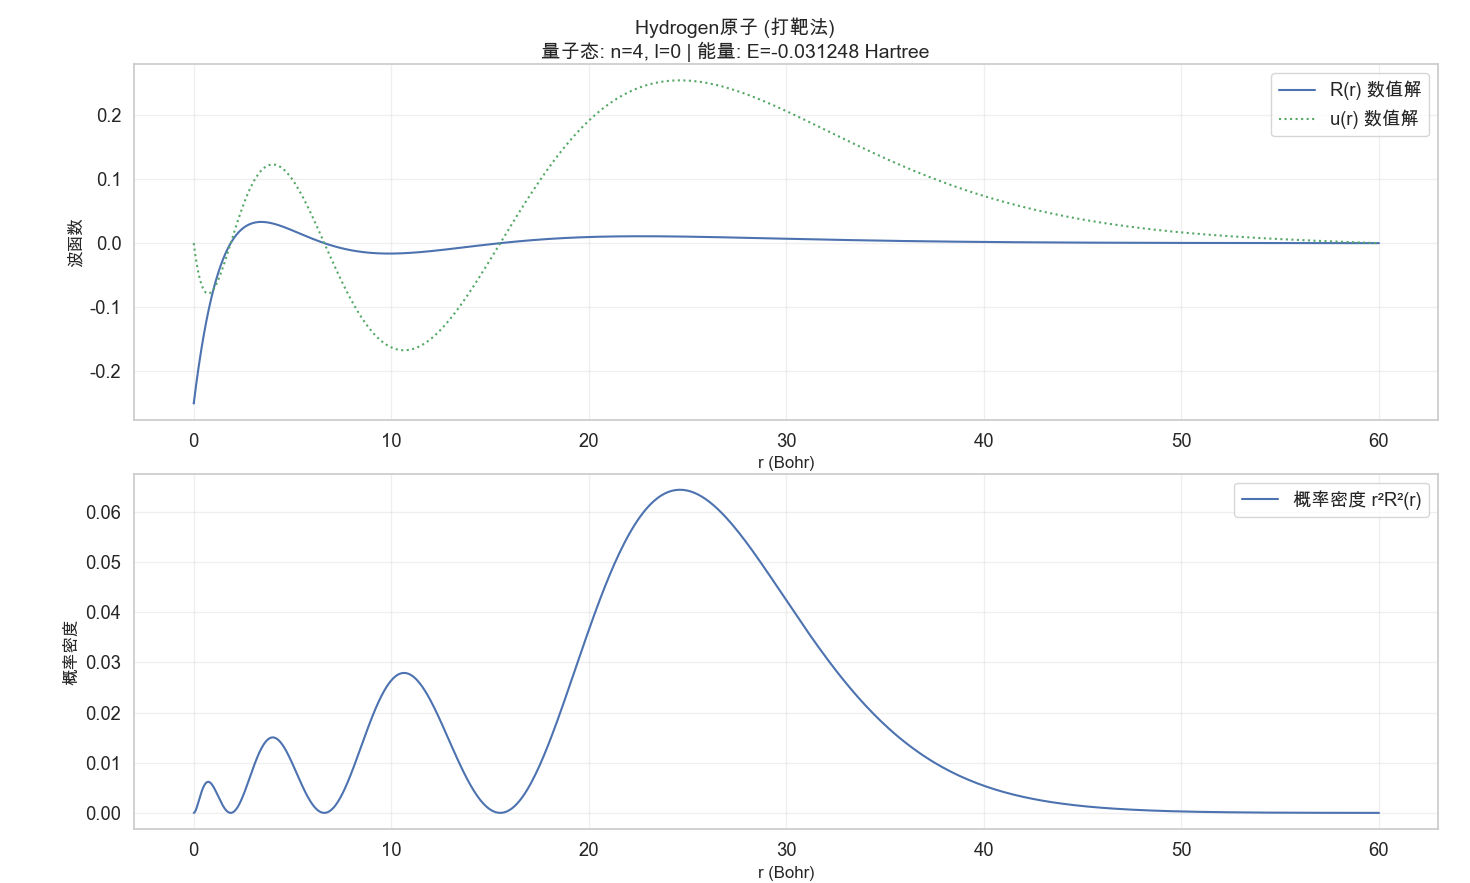
\includegraphics[width=0.6\textwidth]{Problem_2/figs/h_shooting_4s.png}
    \caption{使用打靶法求解氢原子库仑势的4s态,指定\texttt{r\_Max=60}}
\end{figure}

\begin{figure}[H]
    \centering
    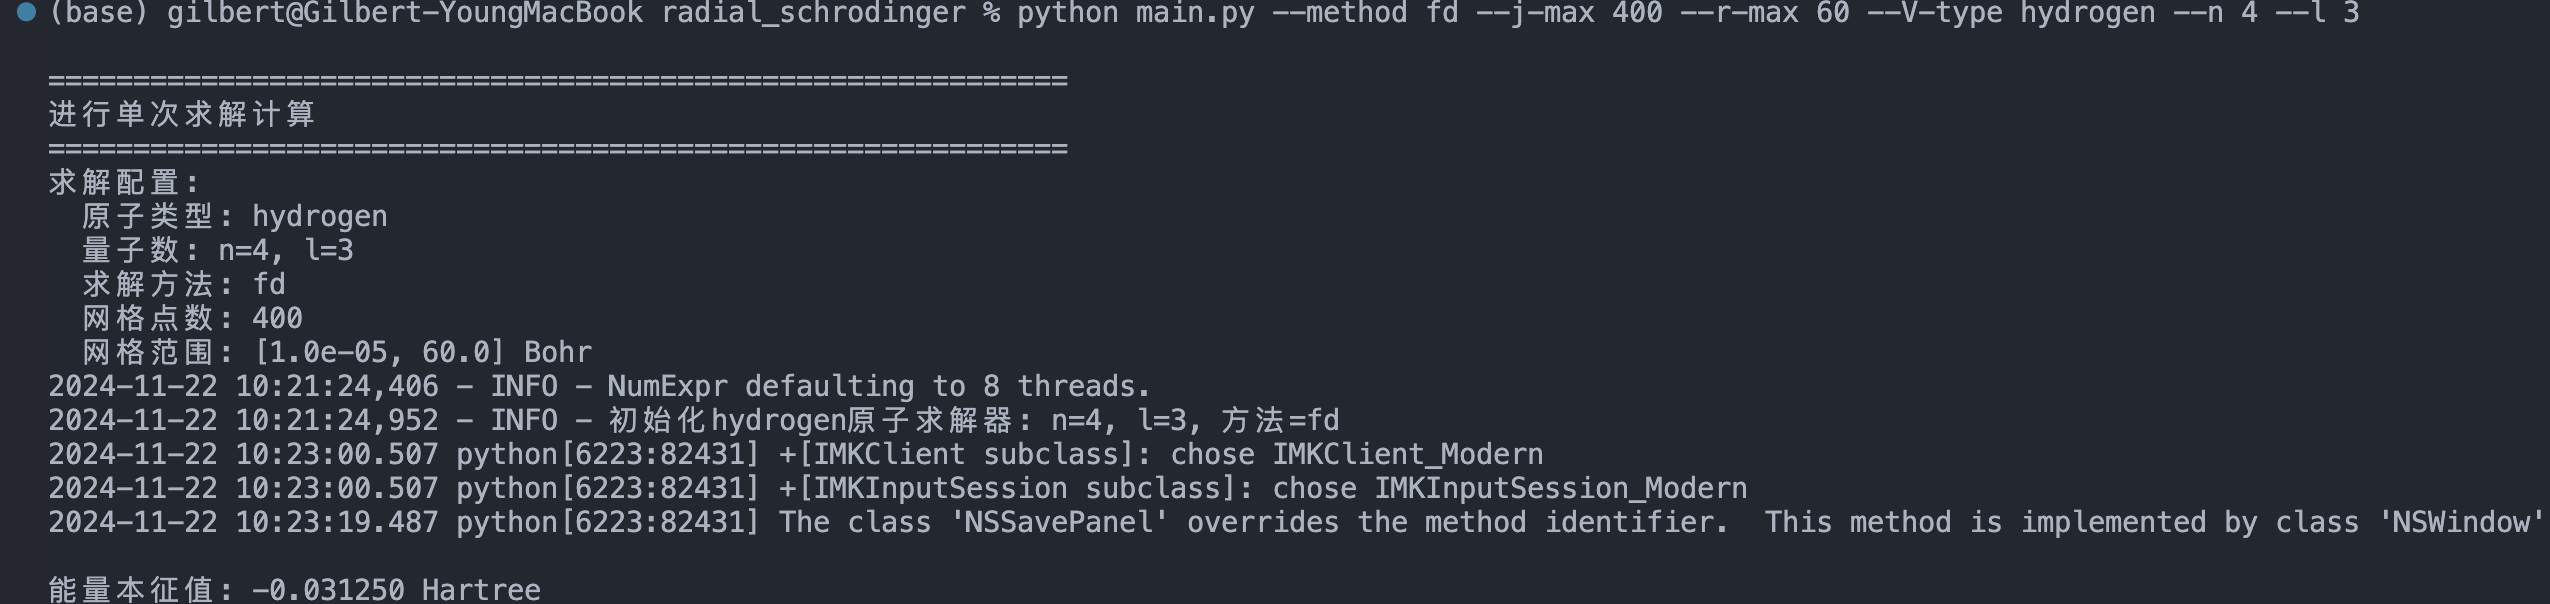
\includegraphics[width=0.6\textwidth]{Problem_2/figs/h_fd_4f_terminal.png}
    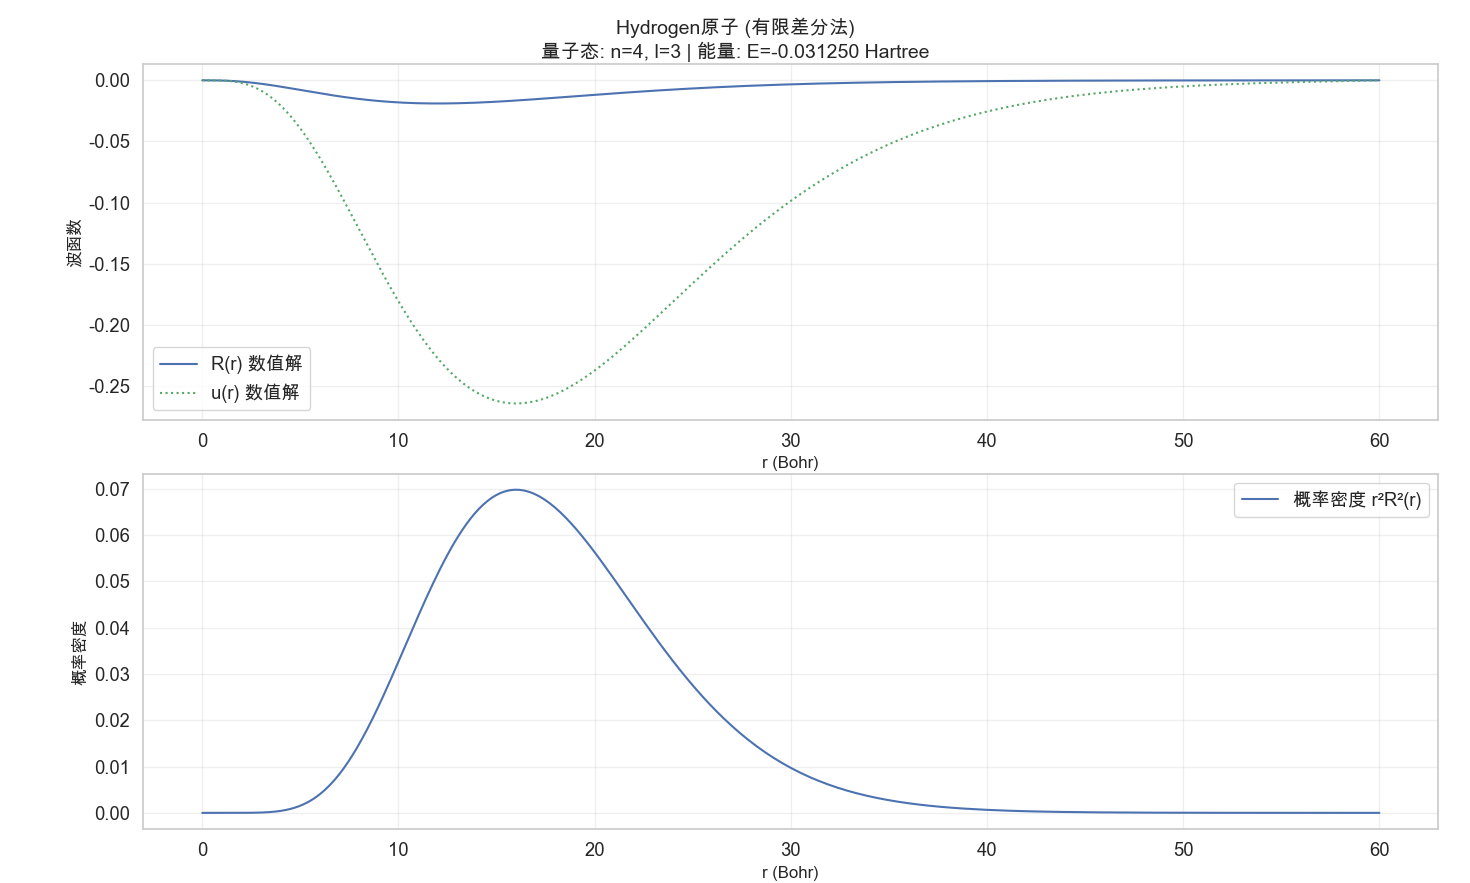
\includegraphics[width=0.6\textwidth]{Problem_2/figs/h_fd_4f.png}
    \caption{使用有限差分法求解氢原子库仑势的4f态,指定\texttt{r\_Max=60}}
\end{figure}

\subsubsection{锂原子其它示例}
\begin{figure}[H]
    \centering
    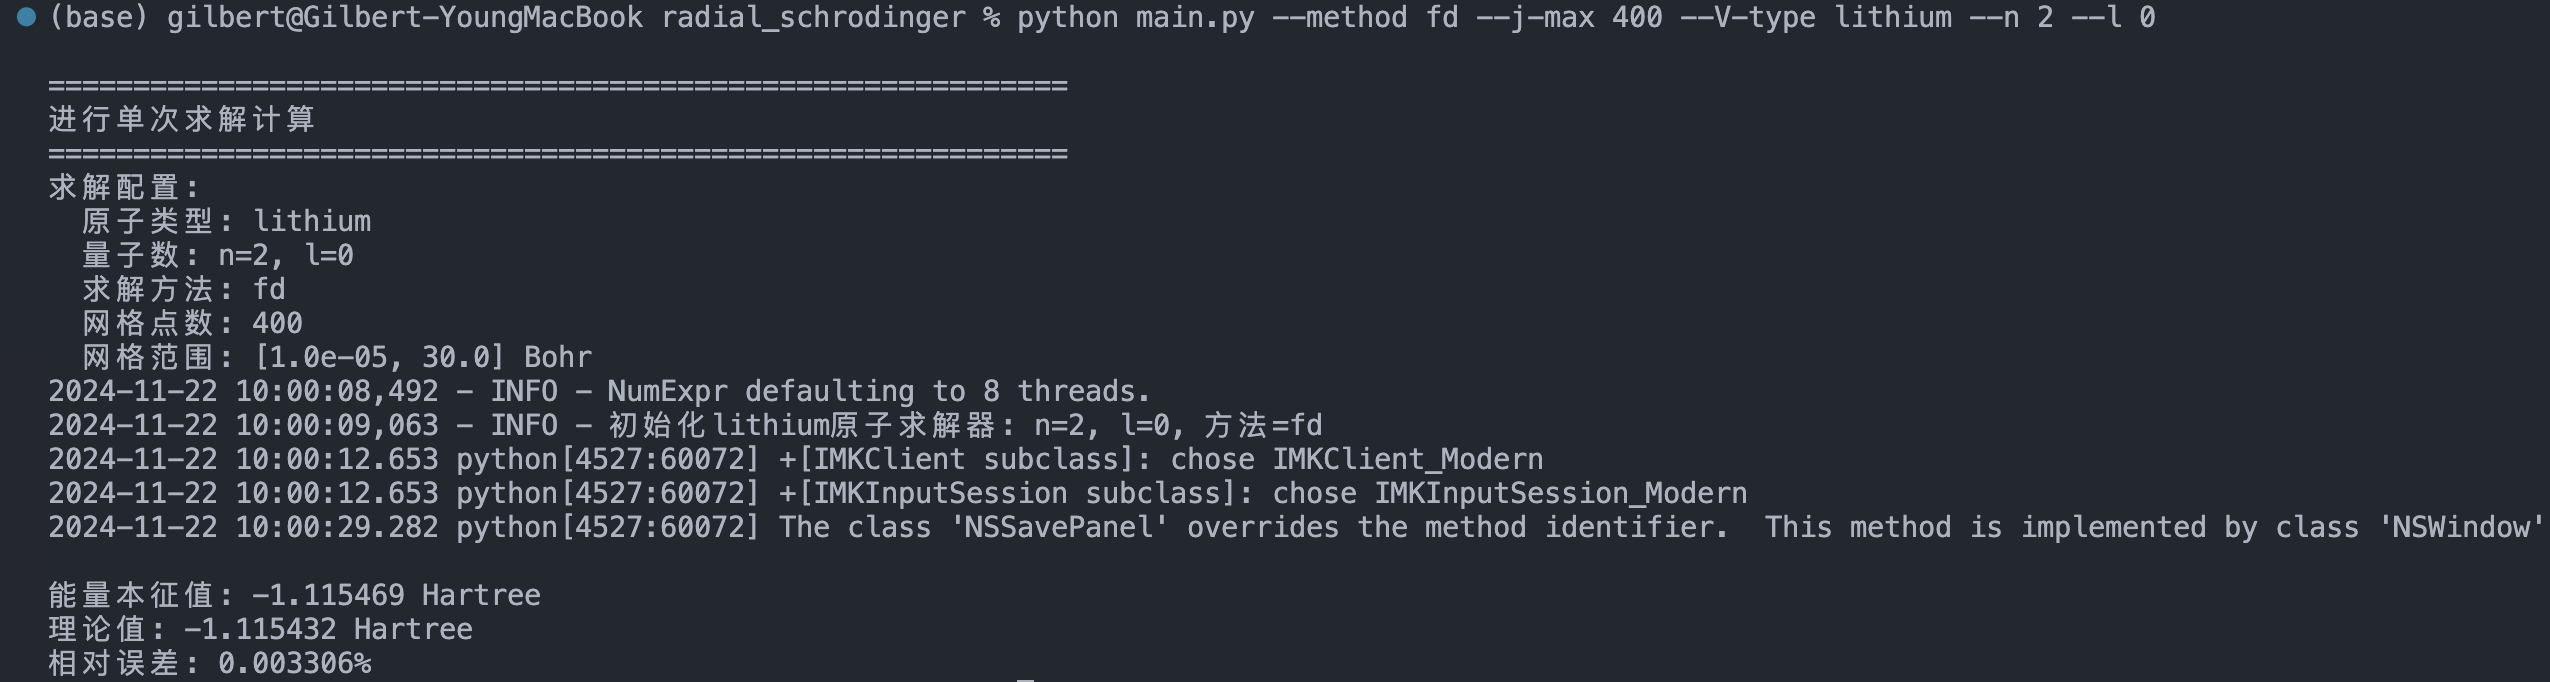
\includegraphics[width=0.6\textwidth]{Problem_2/figs/li_fd_2s_terminal.png}
    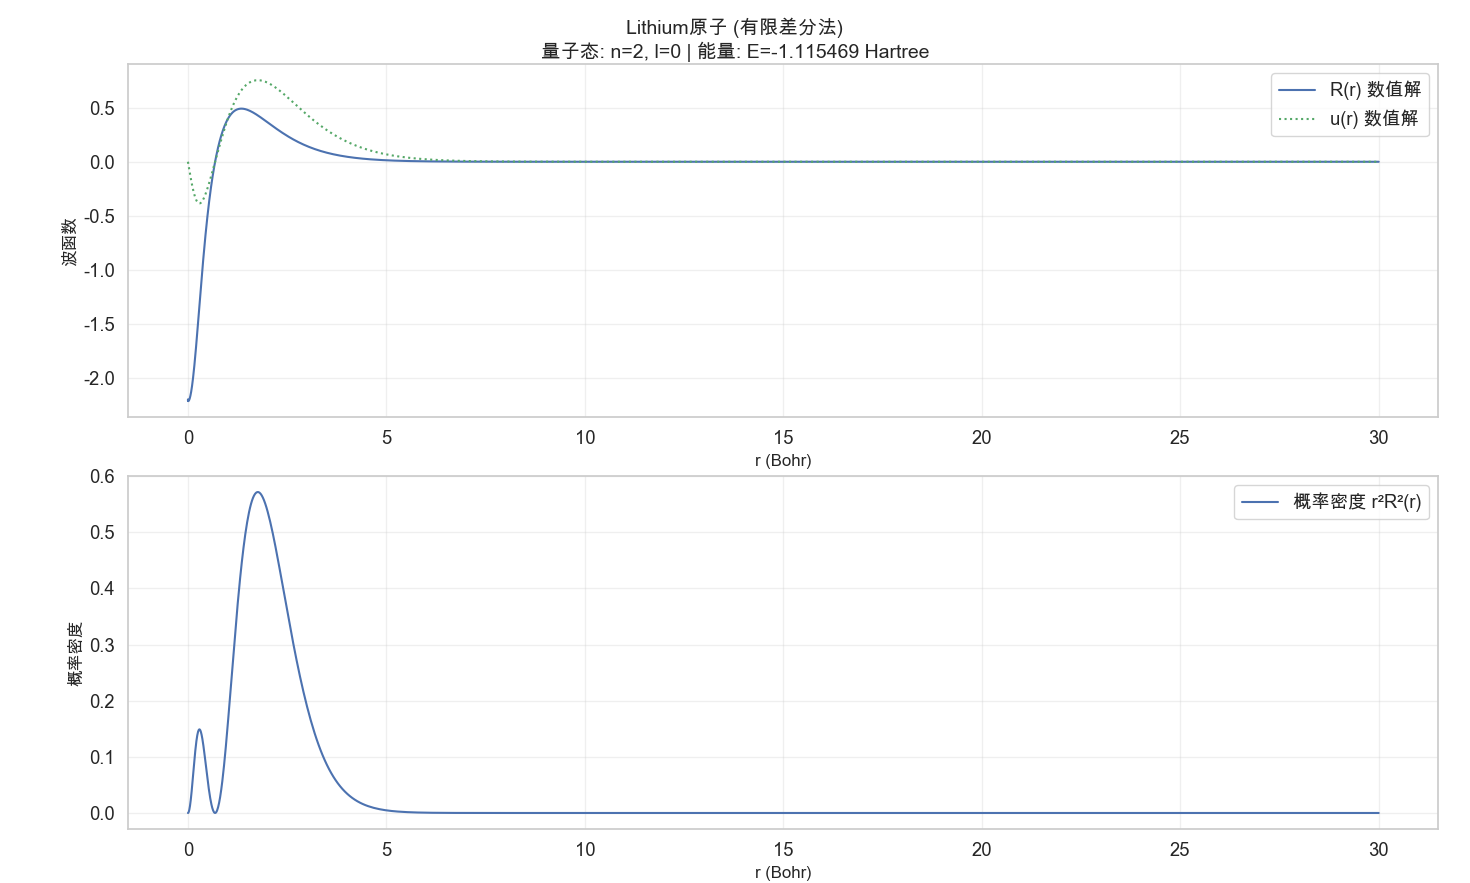
\includegraphics[width=0.6\textwidth]{Problem_2/figs/li_fd_2s.png}
    \caption{使用有限差分法求解锂原子局域势的2s态}
\end{figure}

\begin{figure}[H]
    \centering
    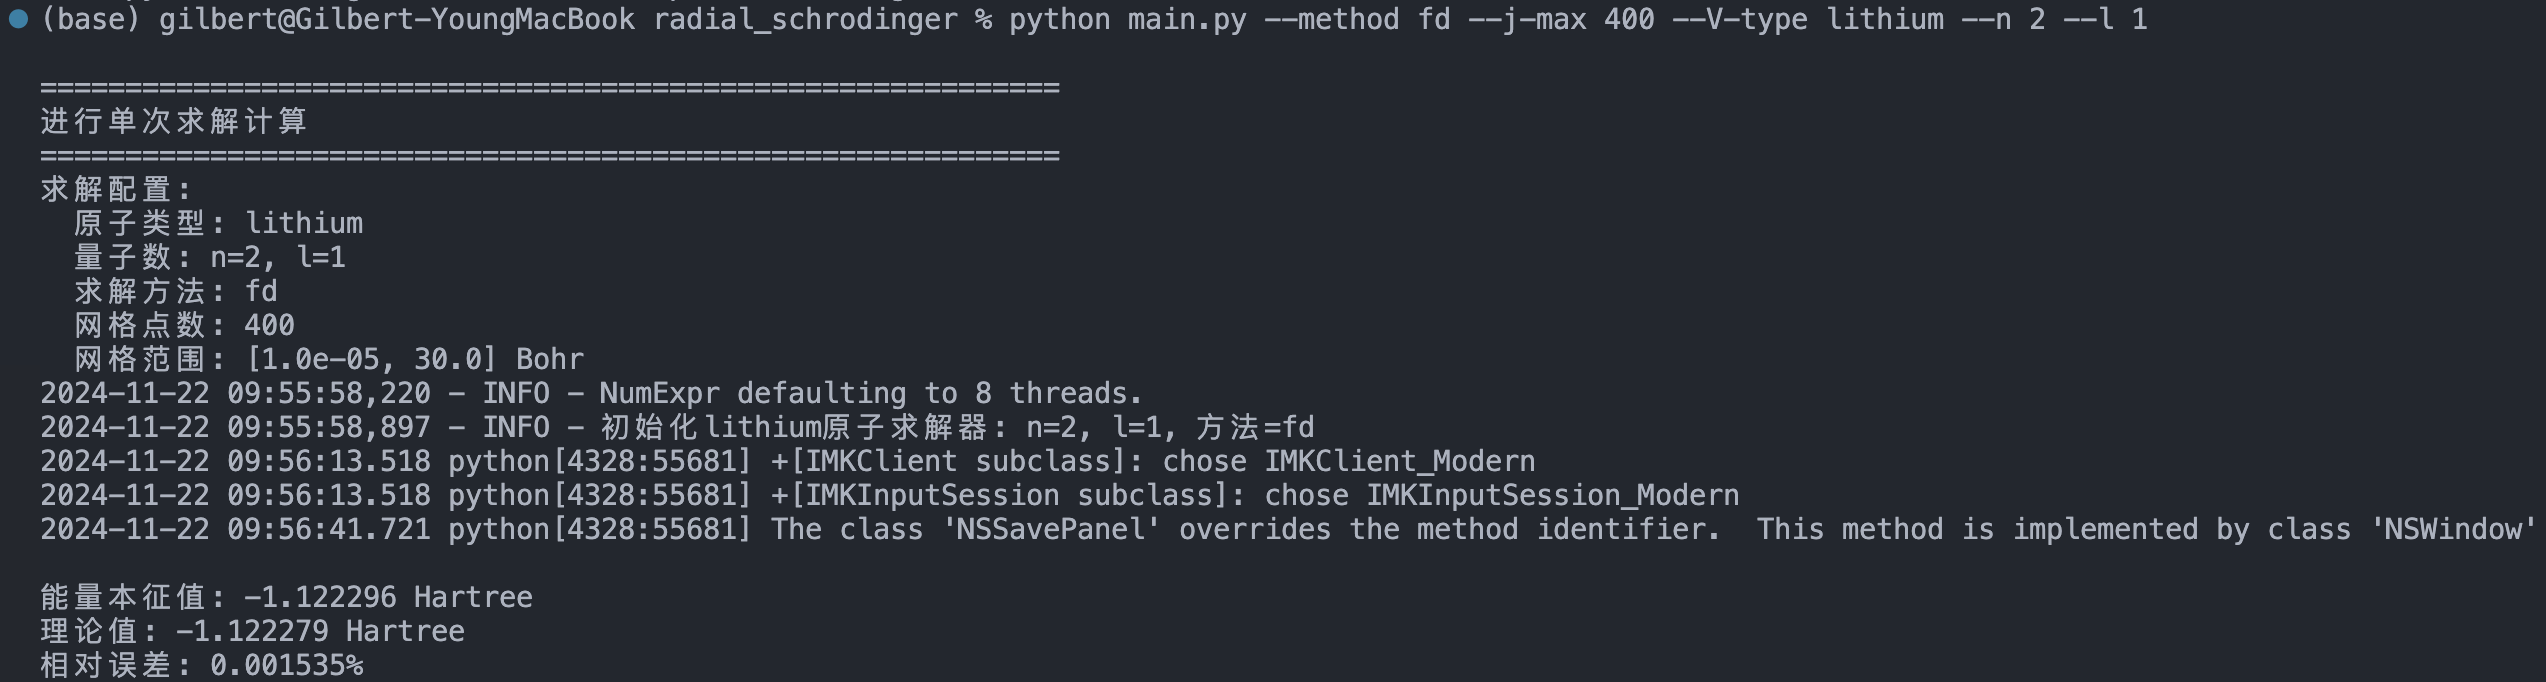
\includegraphics[width=0.6\textwidth]{Problem_2/figs/li_fd_2p_terminal.png}
    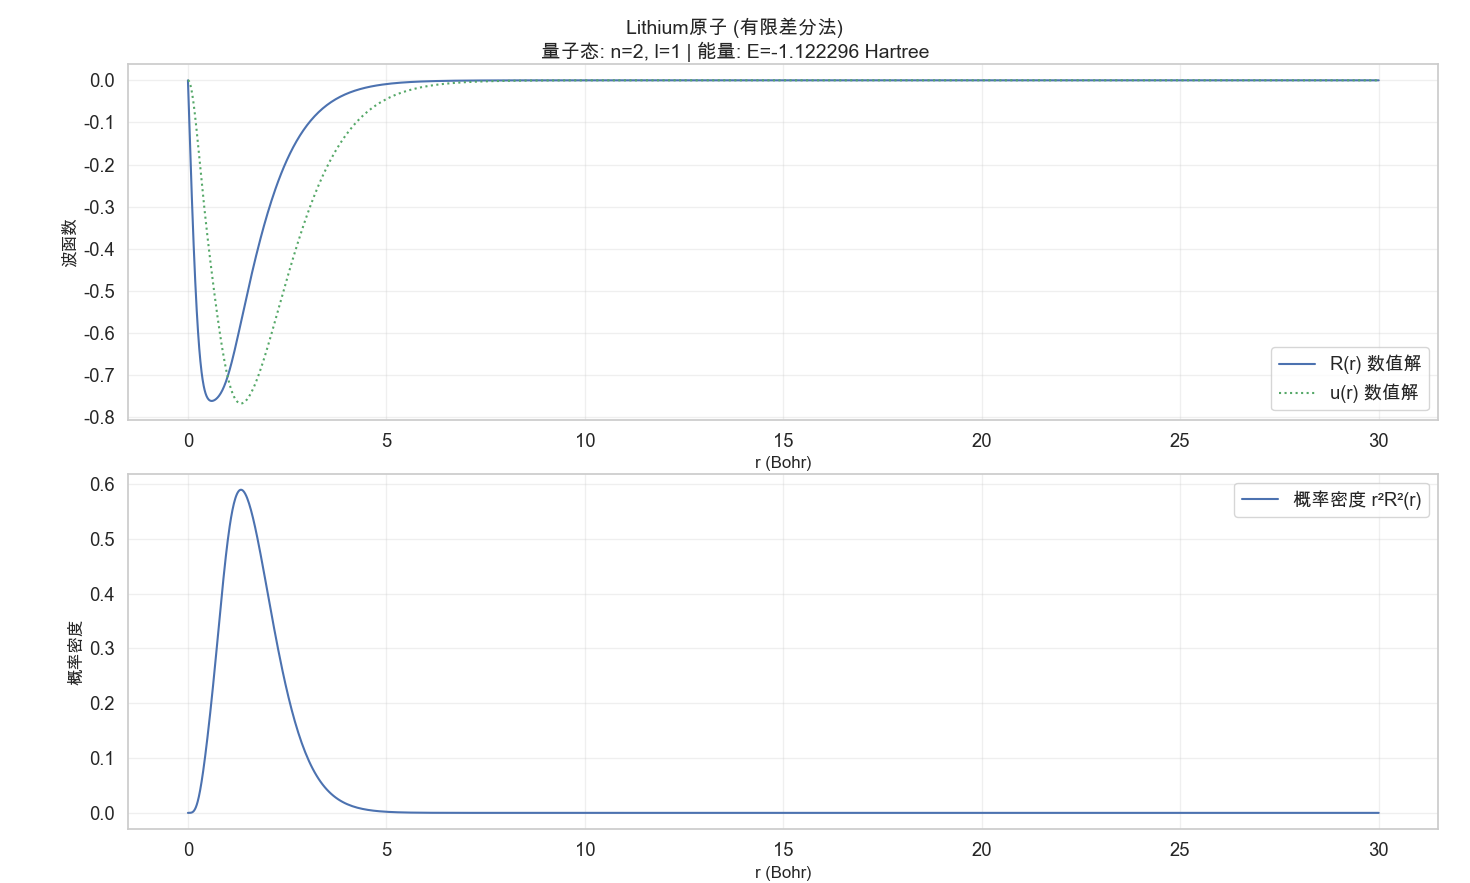
\includegraphics[width=0.6\textwidth]{Problem_2/figs/li_fd_2p.png}
    \caption{使用有限差分法求解锂原子局域势的2p态}
\end{figure}

\begin{figure}[H]
    \centering
    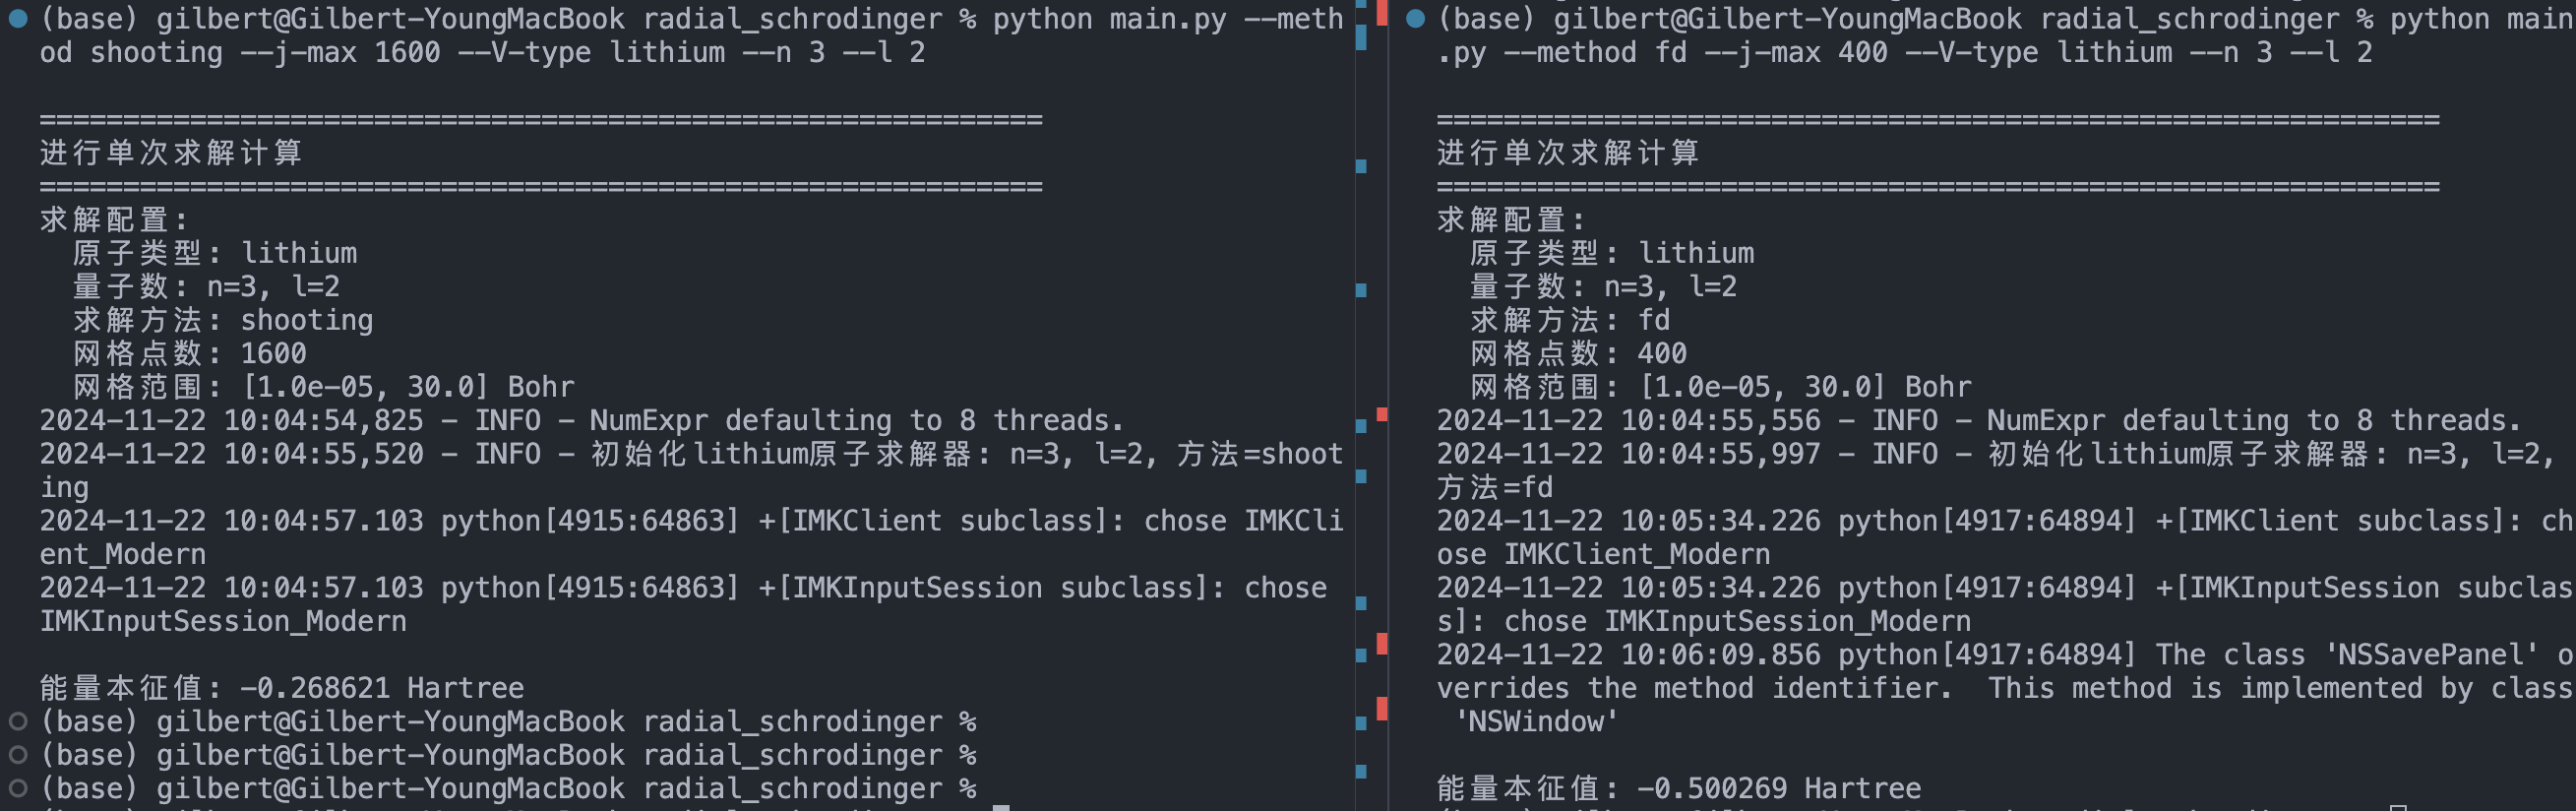
\includegraphics[width=0.8\textwidth]{Problem_2/figs/li_sh&fd_3d_terminal.png}
    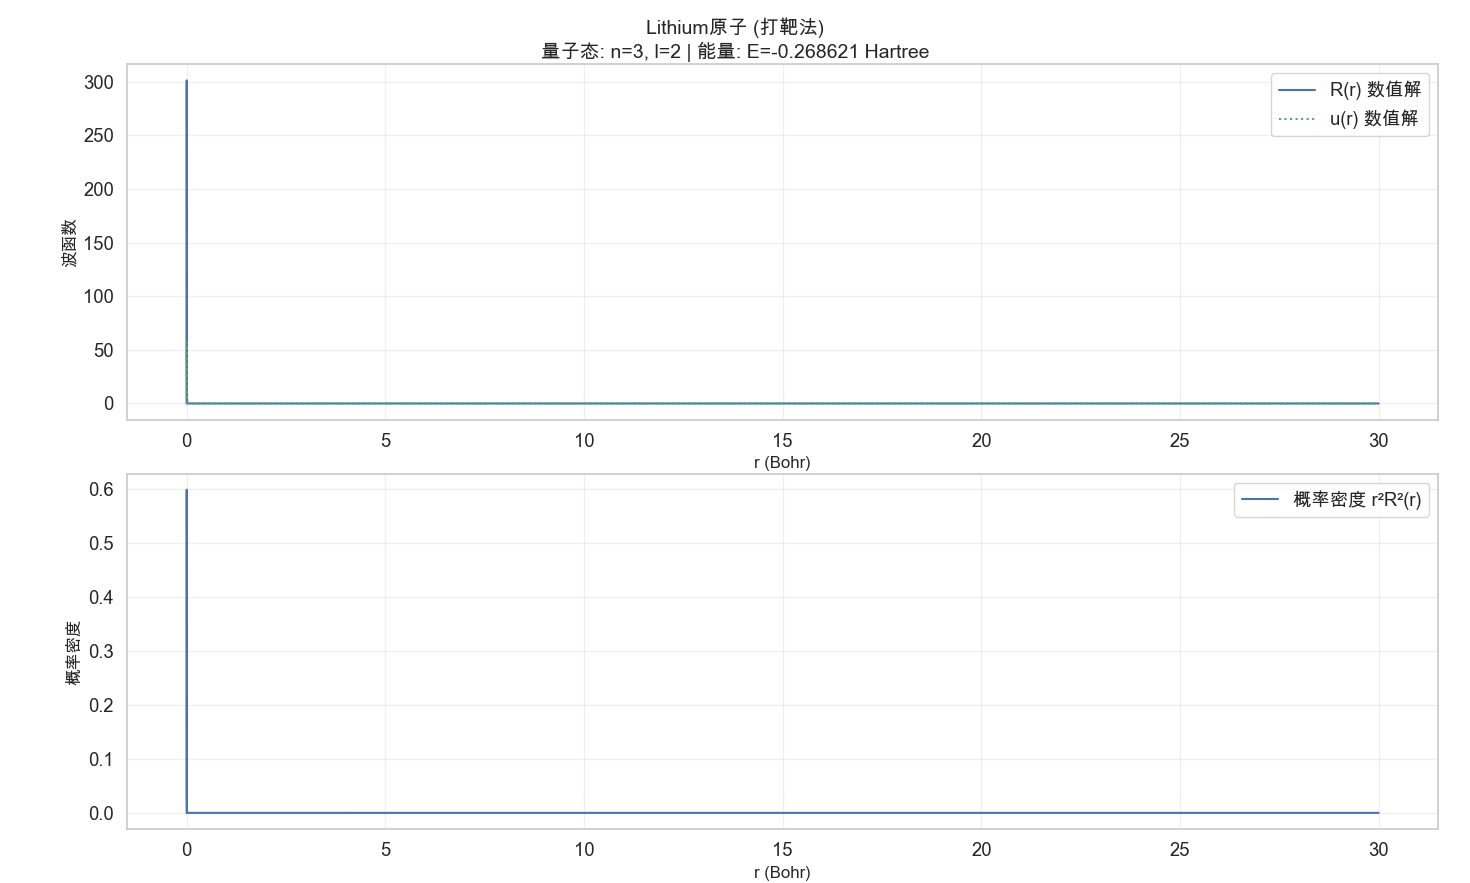
\includegraphics[width=0.8\textwidth]{Problem_2/figs/li_shooting_3d.png}
    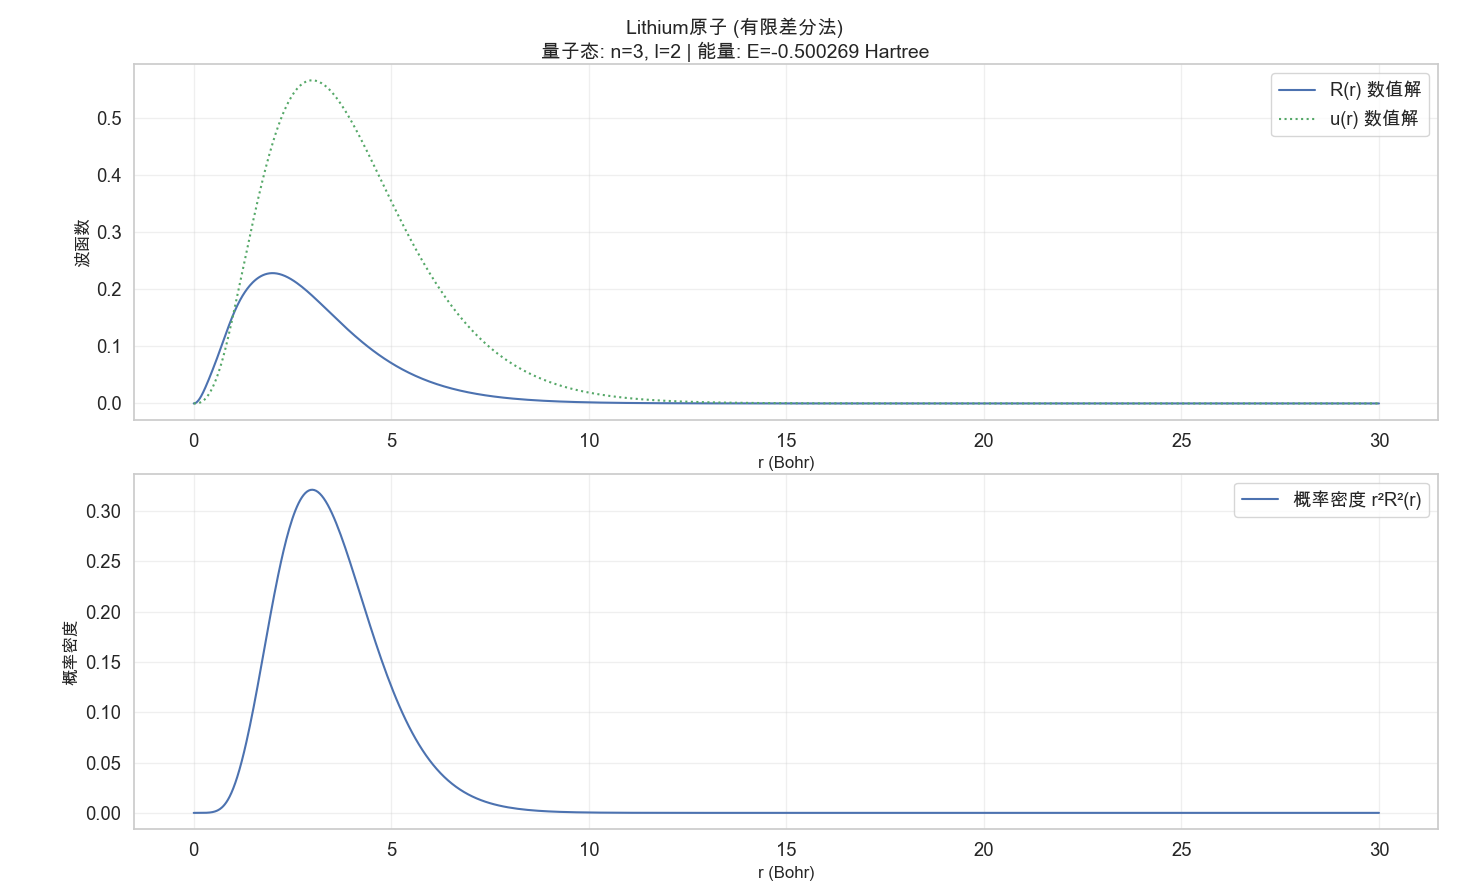
\includegraphics[width=0.8\textwidth]{Problem_2/figs/li_fd_3d.png}
    \caption{分别使用打靶法与有限差分法求解锂原子局域势的3d态,其中打靶法必须拓展\texttt{r\_Max},否则无法收敛}
\end{figure}
